% =====================================================================
% Quantifying Process Model Generalization -- M.Sc. report, LMU Munich.
% LNCS / Springer format. Compile with:
%   pdflatex -enable-installer main_v5 && bibtex main_v5 && pdflatex main_v5 && pdflatex main_v5
% ---------------------------------------------------------------------
% REVISION DRAFT (v5): v4 content (five-log results, M9, AVATAR option C)
% restructured per the supervisor's written feedback of 2026-07:
% subsection-free introduction with a generalization figure, definitions-
% only background, related-work comparison table, formalized method
% (domains for every symbol, config values moved to Sect. 6.1, worked
% toy example), evaluation regrouped into Setup / Results / Discussion /
% Threats, log ids renamed from D-prefix to L1-L5, paragraph-free conclusion.
% The \chg highlighting of v4 is neutralized (renders black).
% main.tex and main_v2/v3/v4.tex are untouched.
% ---------------------------------------------------------------------
% SHORT VERSION (main_v5_short): same content as main_v5, body cut to the
% 20-25 page window. Moved to the appendix: feasibility forensics, the
% per-method calibration figure, the acceptance figure, the genval fold
% table, baseline integration details, the complexity derivation, and the
% Katz-mutation illustration. Related work, the M6 study, and acceptance
% prose are compressed; no result or disclosure is dropped.
% =====================================================================
\documentclass[runningheads]{llncs}

\usepackage[T1]{fontenc}
\usepackage{graphicx}
\usepackage{amsmath}
\usepackage{amssymb}
\usepackage{booktabs}
\usepackage{multirow}
\usepackage{xcolor}
\usepackage{tikz}
\usetikzlibrary{positioning,arrows.meta}
\usepackage{algorithm}
\usepackage{algpseudocode}
\usepackage{listings}
\usepackage[hidelinks]{hyperref}

\emergencystretch=3em
\setcounter{secnumdepth}{3}

% v5: change tracking neutralized; \chg renders as normal text.
\definecolor{chgblue}{RGB}{0,0,0}
\newcommand{\chg}[1]{#1}

\lstset{
  basicstyle=\ttfamily\scriptsize,
  breaklines=true,
  columns=fullflexible,
  keepspaces=true,
  frame=single,
  rulecolor=\color{black!30},
  framesep=4pt,
  xleftmargin=4pt,
  showstringspaces=false
}

\newcommand{\genshadow}{\ensuremath{\mathit{Gen}_{\mathit{shadow}}}}
\newcommand{\genaccept}{\ensuremath{\mathit{Gen}_{\mathit{accept}}}}
\newcommand{\punseen}{\ensuremath{p_{\mathit{unseen}}}}
\newcommand{\pend}{\ensuremath{p_{\mathit{end}}}}
\newcommand{\shlog}{\ensuremath{L_S}}

\begin{document}

\title{Quantifying Process Model Generalization:\\
A Generative N-gram Metric and a Cross-Paradigm Benchmark\thanks{Report, M.Sc.\ Computer Science, LMU Munich.}}
\titlerunning{Quantifying Process Model Generalization}

\author{Christian Daniel Krengel \and Tianhao Geng}
\authorrunning{C.\,D. Krengel and T. Geng}
\institute{Ludwig-Maximilians-Universit\"at M\"unchen, Munich, Germany}

\maketitle

\begin{abstract}
Process discovery derives a process model from an event log, and the discovered model is conventionally judged along four quality dimensions: fitness, precision, simplicity, and generalization. Generalization, the degree to which a model accepts future valid behavior that is absent from the log, is the least validated of the four: published metrics follow incompatible paradigms and are almost never tested against a ground truth on real-life logs. We make four contributions. First, we argue for a strict construct definition: generalization covers only future valid behavior; penalizing invalid behavior is the task of precision. The trace model and the flower model operationalize the two poles and yield a purity litmus. Second, we present \emph{ShadowGen}, a generative metric: a variable-order N-gram model of the log generates a synthetic shadow log of plausible-but-unseen traces, and a model is scored by the graded replay of that shadow log; a strict acceptance reading of the same shadow log anchors the construct poles in validation. Third, we design a benchmark that validates ShadowGen and eight published metrics against a variant-based cross-validation ground truth on four agreement criteria. Fourth, we evaluate on five real-life logs spanning scale, trace depth, and representativeness. ShadowGen tracks the ground truth on every log at a median of $3$ seconds per model, faster than every published baseline. The metric shipped in the widely used PM4Py library correlates negatively with the ground truth and fails the litmus on every log, and an adapted bootstrap generalization matches our calibration, corroborating the generative approach.

\keywords{Process mining \and Process discovery \and Generalization \and Model quality \and Conformance checking \and Benchmark.}
\end{abstract}

% =====================================================================
\section{Introduction}
\label{sec:intro}

Process discovery algorithms construct process models from event logs recorded by information systems~\cite{vanderaalst2016pm}. A discovered model is conventionally assessed along four quality dimensions~\cite{buijs2014quality}: \emph{fitness} (the model allows observed valid behavior), \emph{precision} (it does not allow invalid behaviors), \emph{simplicity} (it is structurally sparse) and \emph{generalization} (it allows future valid behavior). An event log is only a sample of an underlying process: it contains the traces that were recorded, not all traces the process can produce. Generalization captures whether a model describes the process rather than memorizing the sample. Figure~\ref{fig:venn} shows the three sets involved: the behavior of the system, the behavior of the model, and the log that samples the former.

\begin{figure}[t]
\centering
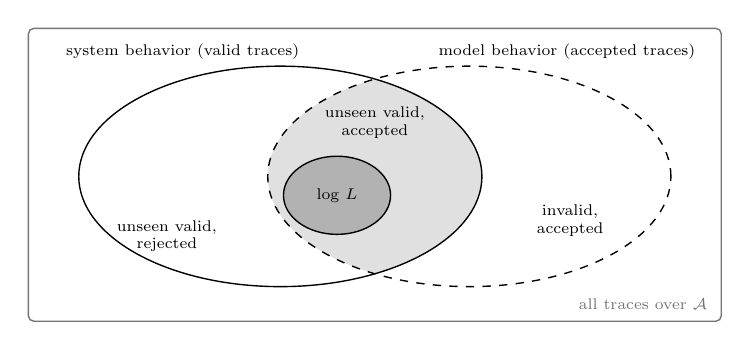
\begin{tikzpicture}[font=\scriptsize, line width=0.5pt, scale=0.80, every node/.style={transform shape}]
  \draw[rounded corners=2pt, color=black!55] (0,0) rectangle (11.0,4.65);
  \node[anchor=south east, color=black!55] at (10.9,0.06) {all traces over $\mathcal{A}$};
  % shaded lens: model behavior that is also system behavior
  \begin{scope}
    \clip (4.0,2.3) ellipse (3.2 and 1.75);
    \fill[black!12] (7.0,2.3) ellipse (3.2 and 1.75);
  \end{scope}
  \draw (4.0,2.3) ellipse (3.2 and 1.75);
  \draw[dashed] (7.0,2.3) ellipse (3.2 and 1.75);
  % the log: a sample of the system, (mostly) accepted by a discovered model
  \draw[fill=black!30] (4.9,2.0) ellipse (0.85 and 0.62);
  \node at (4.9,2.0) {log $L$};
  \node[align=center] at (2.45,4.28) {system behavior (valid traces)};
  \node[align=center] at (8.55,4.28) {model behavior (accepted traces)};
  \node[align=center] at (5.5,3.15) {unseen valid,\\accepted};
  \node[align=center] at (2.2,1.35) {unseen valid,\\rejected};
  \node[align=center] at (8.6,1.6) {invalid,\\accepted};
\end{tikzpicture}
\caption{Generalization as a set relation. The system produces the valid traces; the log is the observed sample; the model accepts some language of traces. Generalization asks how much of the unseen valid behavior the model accepts (the shaded region outside $L$) and is undermined by the lower-left region (future valid behavior the model rejects). The lower-right region, invalid but accepted behavior, is the concern of precision, not of generalization; replaying $L$ itself is the concern of fitness. Every metric only ever sees $L$, so the two unseen regions must be estimated.}
\label{fig:venn}
\end{figure}

This report is about measuring generalization, not about discovering better models. Most published generalization metrics propose a measure and demonstrate it qualitatively; our stance is validation: a single-shot score is trustworthy only if it agrees with a direct, expensive measurement of generalization (hold-out acceptance). We also adopt a deliberately narrow definition, the acceptance of future valid behavior and nothing else, kept strictly separate from precision; this turns the otherwise-useless flower model into a diagnostic litmus test (Sect.~\ref{sec:method:construct}). Finally, any metric and any hold-out ground truth is computed from a log, so its accuracy is bounded by how representatively the log samples the system~\cite{karunaratne2024representativeness}; we treat representativeness as a property of the data and span it deliberately across our datasets.

Measuring generalization is hard for a simple reason: it makes a claim about behavior that, by definition, is not in the data. The literature offers various metrics, but they approach the problem from fundamentally different angles: counting rarely used model parts~\cite{buijs2014quality}, information-theoretic relevance~\cite{alkhammash2022entropic}, anti-alignments~\cite{vandongen2016anti}, adversarial networks~\cite{theis2020avatar}, bootstrapping~\cite{polyvyanyy2022bootstrap}, negative events~\cite{vandenbroucke2014negative} and species estimation~\cite{kabierski2023species}. These paradigms produce scores that are not clearly commensurable, and generalization metrics, unlike fitness and precision metrics, are known not to agree with one another~\cite{janssenswillen2017comparative}. No prior work validates them across paradigms against an empirical, log-derived generalization ground truth on common real-life logs. The practical consequence: no validated consensus generalization metric exists. Even the generalization measure shipped in PM4Py~\cite{berti2019pm4py}, one of the most widely used process-mining libraries, does not track empirical generalization, as we show. A practitioner therefore has no validated, affordable instrument for the fourth quality dimension.

We pursue two goals. The first is a \emph{new metric}. \emph{ShadowGen}\footnote{The implementation package keeps the legacy name \texttt{HybridGen}, from an earlier design that paired the generative score with a structural term. That term was retired (Sect.~\ref{sec:method:framework}), so the metric here is the pure generative component.} learns a variable-order Markov model of the log: N-grams with Katz-style backoff~\cite{katz1987}. From this, Good--Turing estimation~\cite{gale1995gt} gives a per-context probability that the next event is new. ShadowGen then generates a synthetic \emph{shadow log} of plausible-but-unseen traces and scores a model by how well it replays them~\cite{rozinat2008conformance}. The second goal is a \emph{validated benchmark}. We test ShadowGen and eight published generalization metrics on eight discovery configurations and five real-life logs, and validate each metric against variant-based hold-out (both $k$-fold cross-validation and leave-one-variant-out), which measures acceptance of unseen-but-real behavior directly.

In sum, the contributions are: (i) a strict, precision-free construct definition with an operational purity litmus (Sect.~\ref{sec:method:construct}); (ii) ShadowGen, an interpretable generative metric (Sects.~\ref{sec:method}--\ref{sec:impl}); (iii) a cross-paradigm benchmark anchored by an empirical hold-out ground truth, with both construct poles included and a uniform compute budget (Sect.~\ref{sec:eval}); and (iv) its results on five real-life logs. The headline result: ShadowGen tracks the cross-validation ground truth on every log (Pearson $0.986$--$0.999$) at a median of $3$ seconds per model, while scoring a model artifact in hand, which the ground truth itself cannot; the widely used PM4Py metric is anti-correlated with it on four of five logs and fails the flower litmus on all five.

Sections~\ref{sec:background}--\ref{sec:conclusion} cover, in order: background, related work, the construct and method, the implementation, the benchmark (setup, results, discussion, threats), and the conclusion.

% =====================================================================
\section{Background}
\label{sec:background}
This section fixes the notation and the concepts the report builds on: event logs, process models and their discovery, replay-based conformance, hold-out evaluation, and N-gram language models.

\subsection{Event logs}
Let $\mathcal{A}$ be a finite set of activities. A trace $\sigma=\langle a_1,\dots,a_k\rangle\in\mathcal{A}^{*}$ is a finite sequence of activities; $|\sigma|$ is its length, and $\mathrm{suffix}_n(\sigma)$ denotes the sequence of its last $n$ activities. An event log $L$ is a finite multiset of traces; $|L|$ is the number of traces (cases) it contains. In general, for a multiset $C$ we write $C[x]$ for the multiplicity of $x$ and $|C|=\sum_x C[x]$ for the total count. Traces with an identical activity sequence form a \emph{variant}; we write $V(L)$ for the set of variants and, for a variant $v\in V(L)$, $\#v$ for its case count. Real logs are typically dominated by a few frequent variants and a long tail of rare ones.

\subsection{Process models and discovery}
A process discovery algorithm (a miner, for short) maps an event log to a process model; in this report the model class is accepting Petri nets, and a model's language is the set of traces it accepts. Two extreme constructions bound the model space: a \emph{trace model}, one isolated path per observed variant, accepting exactly the observed variants, and a \emph{flower model}, all activities in a single self-loop, accepting every sequence over $\mathcal{A}$.

\subsection{Token replay and its two readings}
Token-based replay~\cite{rozinat2008conformance} replays a trace on a net, firing transitions and accounting for produced, consumed, missing, and remaining tokens. It yields two distinct quantities that this report keeps separate:
\begin{itemize}
  \item a graded trace fitness in $[0,1]$ derived from the token bookkeeping, which awards partial credit (a trace the net cannot actually execute end-to-end can still score, e.g., $0.7$);
  \item a boolean perfect-replay flag: the trace replays with no missing or remaining tokens, i.e., it is in the model's language.
\end{itemize}
The fitness of a log is the mean trace fitness; the acceptance rate is the fraction of perfectly replayed traces. As Sect.~\ref{sec:eval:accept} shows, the graded and boolean readings can diverge sharply, and the gap between them is itself informative.

\subsection{Hold-out evaluation}
The most direct operationalization of generalization is hold-out evaluation: discover a model on a subset of variants, then measure how well the withheld variants replay. Variant-based $k$-fold cross-validation and leave-one-variant-out realize this at increasing granularity, and cross-validation fitness has been used as a generalization measure when benchmarking discovery algorithms~\cite{augusto2019benchmark}. Hold-out is expensive (leave-one-variant-out requires one discovery per variant) and is only defined when the model can be rediscovered from log subsets, so it evaluates a discovery algorithm rather than a model artifact in hand: ideal as a validation reference, impractical as a routine metric.

\subsection{Variable-order language models}
An N-gram language model predicts the next symbol of a sequence from its preceding context. Two classical techniques make such models robust on sparse data: \emph{Katz backoff}~\cite{katz1987} predicts from the longest recent context that has adequate statistical support, falling back to shorter contexts otherwise, and \emph{Good--Turing estimation}~\cite{gale1995gt} estimates the probability mass of unseen events from the number of singletons (events observed exactly once). Section~\ref{sec:method:gen} instantiates both for event logs.

% =====================================================================
\section{Related Work}
\label{sec:related}

We group published generalization metrics by paradigm. Table~\ref{tab:paradigms} compares them along the two construct questions this report keeps asking: does the metric confront the model with unseen behavior, and what does it blend into the score besides acceptance of valid behavior? The identifiers M2--M9 name the metrics throughout the report; M1 is our own metric. Below we summarize each paradigm, review how such metrics have been evaluated so far, and state the gap.

\begin{table}[t]
\centering
\caption{Published generalization paradigms and this report's metric. ``Blended in'' names what enters the score besides acceptance of unseen valid behavior, the construct of Sect.~\ref{sec:method:construct}.}
\label{tab:paradigms}
\setlength{\tabcolsep}{2.5pt}
\scriptsize
\begin{tabular}{@{}l p{2.25cm} p{3.85cm} p{2.45cm} p{2.45cm}@{}}
\toprule
ID & Paradigm & Judges a model by & Unseen behavior probed & Blended in \\
\midrule
M1 & ShadowGen (this report) & replay of a generated shadow log of unseen traces & yes: recombinations and novel events & nothing (pure acceptance) \\
M2 & structural counting~\cite{buijs2014quality,berti2019pm4py} & how often model parts are visited when replaying the log & no & structure \\
M3 & entropic relevance~\cite{alkhammash2022entropic} & bits to encode the log under a stochastic model & no & fitness and precision \\
M4 & anti-alignments~\cite{vandongen2016anti} & the model's maximally deviating runs & model runs, not future traces & precision (paired measure) \\
M5 & neural / GAN~\cite{theis2020avatar} & F-measure against GAN-sampled traces & yes: GAN samples & precision (F-measure) \\
M6 & bootstrap~\cite{polyvyanyy2022bootstrap} & recall against resampled, crossover-bred traces & partly: recombinations only & nothing (recall); the shipped tool reports an F-measure \\
M7 & species estimation~\cite{kabierski2023species} & coverage profiles of original and simulated logs & no & diversity \\
M8 & pattern-based~\cite{reissner2022pattern} & alignment realization of mined behavioral patterns & no: patterns from the log & structure \\
M9 & negative events~\cite{vandenbroucke2014negative} & replay against artificial negative events & no: negatives from the same log & precision-shaped signal \\
\bottomrule
\end{tabular}
\end{table}

\subsection{The paradigms in brief}
Structural counting (M2), the generalization metric built into PM4Py~\cite{buijs2014quality,berti2019pm4py}, deems a model general when its internal parts are visited often while replaying the log; it never confronts the model with unseen behavior, and alignment-based generalization~\cite{vanderaalst2016pm} shares this blind spot, so we group it with M2. Negative-event generalization (M9) completes the log with events assumed forbidden~\cite{vandenbroucke2014negative}; the negatives are induced from the log itself, which folds a precision-shaped signal into the score. Entropic relevance (M3) measures the bits to encode the log under a stochastic model~\cite{alkhammash2022entropic}; it blends fitness- and precision-like aspects and needs a stochastic model that a plain Petri net does not provide. Earth Mover's Stochastic Conformance~\cite{leemans2019emsc} shares both properties, so we treat both as outside a pure generalization comparison.

Anti-alignments (M4) derive precision and generalization from a model's maximally deviating runs~\cite{vandongen2016anti}; the underlying search is exponential. AVATAR (M5) trains a sequence GAN to approximate the system and scores an F-measure against its samples~\cite{theis2020avatar}; it is the closest paradigm to ours, at hours of GPU training per log, and the F-measure folds precision in. Bootstrap generalization (M6) resamples the log and breeds recombined traces via genetic crossover~\cite{polyvyanyy2022bootstrap}; its target, model--system recall, coincides with our construct and makes it the strongest baseline, but its test traces are recombinations of observed material, never novel events. SpeciAL (M7) transfers species-richness estimation from ecology to event data~\cite{kabierski2023species}; we use the coverage ratio between model-simulated and original logs as its generalization proxy. Pattern-based generalization (M8) mines behavioral patterns from the log and checks, via alignments, whether the model realizes them with generalizing structures~\cite{reissner2022pattern}.

\subsection{Membership versus graded semantics}
Textbook definitions are membership-shaped (the likelihood that previously unseen but valid behavior is allowed~\cite{vanderaalst2016pm}; yes/no per trace), whereas token- and alignment-based fitness made the prevailing practice graded~\cite{rozinat2008conformance}. Our metric reports both readings of the shadow log and validates each against its own ground truth.

\subsection{Evaluating the metrics themselves}
A few studies assess the metrics rather than the models. Janssenswillen et al.~\cite{janssenswillen2017comparative} found that, unlike fitness and precision, generalization metrics \emph{do not agree with one another}, and a follow-up on synthetic known-system logs judged objective measurement ``nearly impossible''~\cite{janssenswillen2019confirmatory}. Others check conformance measures against axioms~\cite{vanderaalst2018propositions,syring2019conformance} or benchmark discovery algorithms using these metrics as given~\cite{augusto2019benchmark}.

\subsection{The gap, and how ShadowGen differs}
Three gaps recur. First, no cross-paradigm validation: metrics have been compared to one another~\cite{janssenswillen2017comparative} or on synthetic known-system data~\cite{janssenswillen2019confirmatory}, never against an empirical hold-out ground truth on common real logs, so it is unknown which paradigm actually tracks held-out acceptance. Second, opacity: the most faithful baselines (neural, bootstrap) return a number with little insight into why a model scored as it did. Third, construct drift: several metrics fold precision in (Table~\ref{tab:paradigms}, last column), which conflates two orthogonal failure modes. ShadowGen differs from every other row of the table in combining three properties: it is validated against a cross-validation ground truth and shown to track it; it is interpretable, exposing per-context novelty, mutation flags, an openness profile, and a strict acceptance reading; and it is construct-pure by design, with a benchmark that makes construct drift visible through the flower-model litmus.

% =====================================================================
\section{Method}
\label{sec:method}
This section defines the construct ShadowGen measures (Sect.~\ref{sec:method:construct}), the scoring framework (Sect.~\ref{sec:method:framework}), the generator (Sect.~\ref{sec:method:gen}), its pseudocode (Sect.~\ref{sec:method:algo}), a worked example (Sect.~\ref{sec:method:example}), the complexity (Sect.~\ref{sec:method:complexity}), and the assumptions and limitations of the approach (Sect.~\ref{sec:method:scope}).

\subsection{Construct: what generalization is and is not}
\label{sec:method:construct}
We adopt a strict construct: \textbf{generalization is the degree to which a model accepts future, valid behavior of the underlying process that is absent from the log, and nothing else.} Generalization is \emph{not} precision. Detecting over-permissiveness (acceptance of \emph{invalid} behavior) is the precision dimension's task. Folding a permissiveness penalty into a generalization score makes any mid-range value ambiguous: one cannot tell ``rejects future valid behavior'' from ``accepts invalid behavior.'' That destroys the diagnostic value of the quality quadrant. Metrics that blend the two (for example, AVATAR's harmonic mean of fitness and precision, an F-measure) measure a legitimate but \emph{different} construct and must not be read as pure generalization.

Two degenerate models operationalize the poles (Fig.~\ref{fig:poles}). The \emph{flower model} accepts every sequence over $\mathcal{A}$; its generalization is maximal \emph{by definition}, and it is a useless model because of its precision and simplicity, not its generalization. A pure generalization metric must therefore score it $\approx 1$. The \emph{trace model} memorizes observed variants and accepts nothing unseen; it is the $0$ pole. This yields a \emph{construct-purity litmus}: a metric that scores the flower model below $1$ demonstrably mixes precision or structure into its score. The metric is meant to be read \emph{alongside} precision: a model with $\mathit{Gen}\approx 1$ and precision $\approx 0$ is diagnosed as over-permissive by the precision column, exactly where that information belongs.

\begin{figure}[t]
\centering
\scalebox{0.72}{%
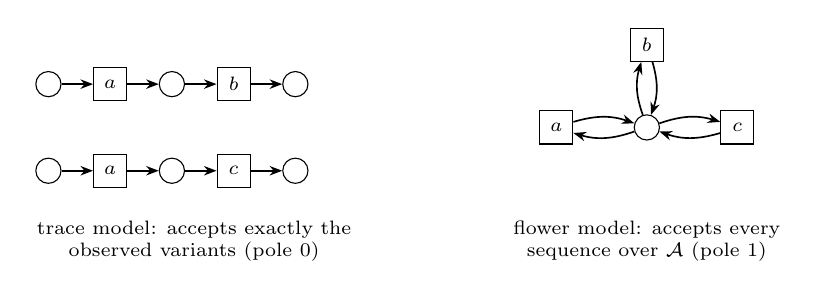
\begin{tikzpicture}[
  font=\scriptsize,
  place/.style={circle, draw, minimum size=3.2mm, inner sep=0pt},
  trans/.style={rectangle, draw, minimum width=4.2mm, minimum height=4.2mm, inner sep=1pt},
  arr/.style={-{Stealth[length=1.6mm]}, semithick}
]
% trace model for the variants <a,b> and <a,c>: one isolated path each
\begin{scope}
  \node[place] (p0) at (0,0.55) {};
  \node[trans, right=4mm of p0] (t1) {$a$};
  \node[place, right=4mm of t1] (p1) {};
  \node[trans, right=4mm of p1] (t2) {$b$};
  \node[place, right=4mm of t2] (p2) {};
  \node[place] (q0) at (0,-0.55) {};
  \node[trans, right=4mm of q0] (u1) {$a$};
  \node[place, right=4mm of u1] (q1) {};
  \node[trans, right=4mm of q1] (u2) {$c$};
  \node[place, right=4mm of u2] (q2) {};
  \draw[arr] (p0) -- (t1); \draw[arr] (t1) -- (p1); \draw[arr] (p1) -- (t2); \draw[arr] (t2) -- (p2);
  \draw[arr] (q0) -- (u1); \draw[arr] (u1) -- (q1); \draw[arr] (q1) -- (u2); \draw[arr] (u2) -- (q2);
  \node[align=center] at (1.85,-1.45) {trace model: accepts exactly the\\observed variants (pole $0$)};
\end{scope}
% flower model over {a,b,c}
\begin{scope}[xshift=7.6cm]
  \node[place] (c) at (0,0) {};
  \node[trans] (fa) at (-1.15,0) {$a$};
  \node[trans] (fb) at (0,1.05) {$b$};
  \node[trans] (fc) at (1.15,0) {$c$};
  \draw[arr] (c) to[bend left=18] (fa); \draw[arr] (fa) to[bend left=18] (c);
  \draw[arr] (c) to[bend left=18] (fb); \draw[arr] (fb) to[bend left=18] (c);
  \draw[arr] (c) to[bend left=18] (fc); \draw[arr] (fc) to[bend left=18] (c);
  \node[align=center] at (0,-1.45) {flower model: accepts every\\sequence over $\mathcal{A}$ (pole $1$)};
\end{scope}
\end{tikzpicture}}
\caption{The two construct poles for a log with variants $\langle a,b\rangle$ and $\langle a,c\rangle$ over $\mathcal{A}=\{a,b,c\}$. The trace model memorizes the variants and accepts nothing unseen; the flower model accepts everything, so a construct-pure metric must score it $1$ (its uselessness is a precision and simplicity verdict, not a generalization verdict).}
\label{fig:poles}
\end{figure}

\subsection{Framework}
\label{sec:method:framework}
ShadowGen scores a model by the replay quality of a synthetic \emph{shadow log}: traces that are plausible under the log's behavior but, by construction, absent from it. The generator is derived from the log alone, and the model under evaluation is consulted only at replay time (Fig.~\ref{fig:pipeline}). This keeps the generation independent of the artifact being judged.

\begin{figure}[t]
\centering
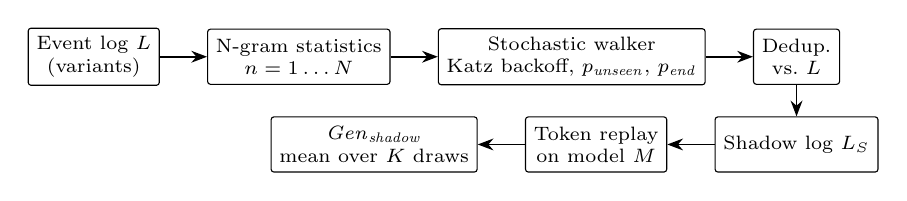
\begin{tikzpicture}[
  node distance=4mm and 6mm,
  box/.style={draw, rounded corners=1pt, align=center, font=\scriptsize, inner sep=3pt, minimum height=7mm},
  arr/.style={-{Stealth[length=2mm]}, semithick}
]
\node[box] (log) {Event log $L$\\(variants)};
\node[box, right=of log] (stats) {N-gram statistics\\$n = 1 \dots N$};
\node[box, right=of stats] (walk) {Stochastic walker\\Katz backoff, $\punseen$, $\pend$};
\node[box, right=of walk] (dedup) {Dedup.\\vs.\ $L$};
\node[box, below=of dedup] (shadow) {Shadow log $\shlog$};
\node[box, left=of shadow] (replay) {Token replay\\on model $M$};
\node[box, left=of replay] (score) {\genshadow\\mean over $K$ draws};
\draw[arr] (log) -- (stats);
\draw[arr] (stats) -- (walk);
\draw[arr] (walk) -- (dedup);
\draw[arr] (dedup) -- (shadow);
\draw[arr] (shadow) -- (replay);
\draw[arr] (replay) -- (score);
\end{tikzpicture}
\caption{ShadowGen pipeline. From the variants of the event log $L$, N-gram statistics up to order $N$ feed a stochastic walker (Katz backoff; novelty probability $\punseen$; termination probability $\pend$). Generated traces are deduplicated against $L$, so the shadow log $\shlog$ contains only unseen traces. The model $M$ under evaluation enters only at the replay step, which yields the metric: the graded score \genshadow{}, averaged over $K$ draws. A strict acceptance reading of the same shadow log (\genaccept) exists as a validation diagnostic (Sect.~\ref{sec:eval:accept}), not as part of the released metric.}
\label{fig:pipeline}
\end{figure}

\subsection{Shadow log generation}
\label{sec:method:gen}
The generator is presented in walk order: the statistics it precomputes, the backoff that resolves a context, the novelty estimate, the mutation proposal, the exploitation step, termination, and the scoring of the finished shadow log.

\subsubsection{Variant statistics.}
The log is compressed to its variants with case counts; every count below is weighted by how often the variant occurs ($\#v$). Let $N\in\mathbb{N}$ be the context bound (an upper limit on the order, not a fixed operating point; its value, like every parameter value, is set in the evaluation protocol, Sect.~\ref{sec:eval:setup}). For each order $n\in\{1,\dots,N\}$ and each observed context $s$ (a length-$n$ activity sequence), we record the successor multiset $C_n(s)$, where $C_n(s)[a]$ is the frequency with which activity $a$ follows $s$, together with its support set $A_n(s)=\{a\in\mathcal{A}:C_n(s)[a]>0\}$, and the termination counts: $T_n(s)$, the number of occurrences of $s$, and $E_n(s)$, the number of those occurrences at the end of a trace. Where the order is clear from the context length we drop the subscript and write $C(s)$, $A(s)$, $T(s)$, $E(s)$.

\subsubsection{Katz backoff.}
At generation time the walker holds a partial trace $\sigma$ and resolves its decision context to the deepest order with adequate support. Let $\tau\in\mathbb{N}$ be a support threshold. The \emph{resolved order} $R$ is the largest $n\le N$ such that the suffix $s=\mathrm{suffix}_n(\sigma)$ satisfies $|C_n(s)|\ge\tau$ (at least $\tau$ observed successor occurrences, Sect.~\ref{sec:background}) \emph{and} the Good--Turing mass below is $<1$. If no order qualifies, the walker falls back to $n{=}1$. $N$ is therefore an upper bound: on sparse logs the effective order is reduced naturally.

\subsubsection{Good--Turing novelty.}
For the resolved context $s$, the probability that the next activity is one never observed after $s$ is estimated as
\begin{equation}
\punseen(s) \;=\; \frac{N_1(s)}{\,|C(s)|\,}, \qquad N_1(s) = |\{a \in A(s) : C(s)[a]=1\}|,
\label{eq:gt}
\end{equation}
i.e., the number of singleton successors over the total successor count. With probability $\punseen(s)$ the walker \emph{mutates}; otherwise it \emph{exploits}.

\subsubsection{Mutation proposal (Katz-consistent).}
When a mutation fires, the inserted activity must be novel in the resolved context yet plausible. We draw it from the deepest \emph{shorter} context that offers a successor unseen at the resolved order $R$. Formally, we take the largest order $m\in\{1,\dots,\min(|\sigma|,N)\}$ whose candidate set
\begin{equation}
B_m \;=\; A_m(\mathrm{suffix}_m(\sigma))\setminus A_R(s)
\label{eq:proposal}
\end{equation}
is nonempty, and sample the inserted activity from $B_m$ (weighted as in the exploitation step below). If no such $m$ exists, we fall back to the global activity frequencies restricted to $\mathcal{A}\setminus A_R(s)$. A short observation shows that this search is a genuine backoff. Every occurrence of a context is also an occurrence of its shorter suffixes with the same next activity, so support sets can only grow as the context shortens: $A_n(\mathrm{suffix}_n(\sigma))\subseteq A_m(\mathrm{suffix}_m(\sigma))$ for $m\le n$. Orders $\ge R$ therefore never offer a candidate outside $A_R(s)$, and the first candidates appear at order $R{-}1$ or below, one level below the resolved order.

\subsubsection{Exploitation: two sampling modes.}
For a non-mutation step the walker samples a seen successor $a\in A(s)$ with probability proportional to $w(c)$, where $c=C(s)[a]$ is the observed successor count and $w:\mathbb{N}\to\mathbb{R}_{\ge0}$ is a weighting function. We support two weighting functions:
\begin{equation}
w_{\mathrm{mle}}(c)=c \qquad\text{vs.}\qquad w_{\mathrm{log}}(c)=\ln(c+1).
\end{equation}
The \texttt{mle} mode samples from the maximum-likelihood estimate of the next-activity distribution (proportional to observed frequency), so the shadow log mirrors the \emph{expected} future. The \texttt{log} mode deliberately flattens the distribution, up-weighting rare paths; it is a rare-behavior \emph{stress test}. The \texttt{mle} mode is the default and is what the evaluation reports; the calibration case for it is measured in Sect.~\ref{sec:eval:scale}. The same weighting governs the mutation-proposal sampling, but never the mutation \emph{rate} of Eq.~\eqref{eq:gt}, which always uses raw counts.

\subsubsection{Context-aware termination.}
Whether the walk ends after context $s$ is decided by a termination probability resolved with the same backoff:
\begin{equation}
\pend(s) \;=\; \frac{E(s)}{T(s)}.
\end{equation}
Conditioning termination on the $n$-gram context (rather than the last activity alone) fixes premature termination when activities that legitimately end traces appear early in a generated trace.

\subsubsection{Deduplication and scoring.}
Each generated trace is compared against the set of original variants and regenerated if it is a copy (up to a retry cap), so the shadow log contains only unseen sequences. A shadow log $\shlog$ of $\theta\in\mathbb{N}$ traces ($\theta$ capped by $|L|$) is replayed on the model; generation and replay are repeated $K\in\mathbb{N}$ times and the scores averaged. The metric is \genshadow{}: the mean graded trace fitness of the shadow log. It is also reported separately for shadow traces that contain a mutation and those that do not, which shows how a model handles genuinely novel events versus mere recombinations. A strict companion reading, \genaccept{} (the fraction of perfectly replayed shadow traces), is computed by the benchmark harness as a validation diagnostic that anchors the construct poles (Sect.~\ref{sec:eval:accept}); it is not part of the released metric.

\subsection{Algorithm}
\label{sec:method:algo}
Algorithm~\ref{alg:gen} gives the generation procedure; statistics gathering and scoring are described above. The function $\mathrm{rand}()$ draws a fresh uniform random number from $[0,1)$; all draws are seeded (Sect.~\ref{sec:impl:decisions}).

\begin{algorithm}[t]
\caption{Shadow-log generation (one iteration)}
\label{alg:gen}
\begin{algorithmic}[1]
\Require event log $L$; context bound $N\in\mathbb{N}$; support threshold $\tau\in\mathbb{N}$; shadow-log size $\theta\in\mathbb{N}$; length cap $\lambda\in\mathbb{N}$; weighting function $w:\mathbb{N}\to\mathbb{R}_{\ge0}$
\State build $C_n,A_n,T_n,E_n$ for $n=1..N$ from the variants of $L$ (Sect.~\ref{sec:method:gen}); collect the start-activity distribution and the variant set $V(L)$
\State $\shlog\gets\emptyset$
\For{$i=1$ to $\theta$}
  \Repeat
    \State $\sigma\gets\langle\,$sample start activity$\,\rangle$
    \State $\mathit{mut}\gets$ false
    \While{$|\sigma|<\lambda$}
      \State resolve context $s$ and order $R$ by Katz backoff with threshold $\tau$
      \If{$\mathrm{rand}()<\pend(s)$} \textbf{break} \EndIf
      \If{$\mathrm{rand}()<\punseen(s)$ \textbf{and} a novel candidate exists (Eq.~\eqref{eq:proposal})}
        \State append a novel activity from $B_m$, weighted by $w$; $\mathit{mut}\gets$ true
      \Else
        \State append a seen successor $a\in A(s)$, $\propto w(C(s)[a])$; \textbf{break} if dead end
      \EndIf
    \EndWhile
  \Until{$\sigma\notin V(L)$ \textbf{or} retry cap reached}
  \State $\shlog\gets\shlog\cup\{(\sigma,\mathit{mut})\}$
\EndFor
\State \Return $\shlog$
\end{algorithmic}
\end{algorithm}

\subsection{Running example}
\label{sec:method:example}
Figure~\ref{fig:example} works the method end to end on a toy log over $\mathcal{A}=\{a,\dots,e\}$; for this example only, the context bound is $N{=}2$ and the threshold $\tau{=}3$ (the benchmark values are fixed in Sect.~\ref{sec:eval:setup}). The four variants yield the N-gram statistics excerpted in the middle panel. The first generated trace, $\langle a,c,e\rangle$, is a pure recombination: every step is attested (both $c$ after $a$ and $e$ after $c$ occur in the log), the sequence as a whole is unseen, deduplication confirms it is no variant, and it carries $\mathit{mut}=\mathrm{false}$. The second trace shows the mutation machinery. At $\sigma=\langle a,b\rangle$ the resolved order is $R{=}2$, since $|C(\langle a,b\rangle)|=5\ge\tau$, with successors $A_2(\langle a,b\rangle)=\{c,d\}$; the singleton $d$ sets the novelty rate $\punseen=1/5$. When the draw fires, the proposal backs off to the deepest shorter context that offers something new (Eq.~\eqref{eq:proposal}): the order-1 context $\langle b\rangle$ offers $\{c,d,e\}$, so $e$ (novel after $\langle a,b\rangle$, yet attested after $\langle b\rangle$) is inserted, and the trace is flagged $\mathit{mut}=\mathrm{true}$.

\begin{figure}[t]
\centering
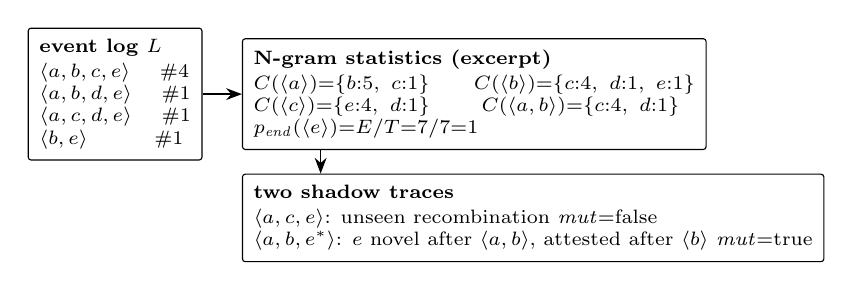
\begin{tikzpicture}[
  node distance=3mm and 5mm,
  box/.style={draw, rounded corners=1pt, align=left, font=\scriptsize, inner sep=4pt},
  arr/.style={-{Stealth[length=2mm]}, semithick}
]
\node[box] (log) {\textbf{event log $L$}\\[1pt]
  $\langle a,b,c,e\rangle$ \quad $\#4$\\
  $\langle a,b,d,e\rangle$ \quad $\#1$\\
  $\langle a,c,d,e\rangle$ \quad $\#1$\\
  $\langle b,e\rangle$ \quad\quad\ \ $\#1$};
\node[box, right=of log] (stats) {\textbf{N-gram statistics (excerpt)}\\[1pt]
  $C(\langle a\rangle){=}\{b{:}5,\ c{:}1\}$\qquad $C(\langle b\rangle){=}\{c{:}4,\ d{:}1,\ e{:}1\}$\\
  $C(\langle c\rangle){=}\{e{:}4,\ d{:}1\}$\qquad\ $C(\langle a,b\rangle){=}\{c{:}4,\ d{:}1\}$\\
  $\pend(\langle e\rangle){=}E/T{=}7/7{=}1$};
\node[box, below=of stats.south west, anchor=north west] (out) {\textbf{two shadow traces}\\[1pt]
  $\langle a,c,e\rangle$: unseen recombination \hfill $\mathit{mut}{=}\mathrm{false}$\\
  $\langle a,b,e^{*}\rangle$: $e$ novel after $\langle a,b\rangle$, attested after $\langle b\rangle$ \hfill $\mathit{mut}{=}\mathrm{true}$};
\draw[arr] (log) -- (stats);
\draw[arr] ([xshift=10mm]stats.south west) -- ([xshift=10mm]out.north west);
\end{tikzpicture}
\caption{Worked example ($N{=}2$, $\tau{=}3$). A toy log of four variants, the successor multisets its N-grams induce, and two generated shadow traces: a recombination of attested steps, and a Katz-consistent mutation ($e^{*}$) whose rate came from the resolved order-2 context and whose proposal came from the order-1 context.}
\label{fig:example}
\end{figure}

The same two-job split of backoff holds at realistic counts: an over-sparse deep context is skipped entirely, the deepest supported order sets how often to invent an event (the rate), and a still shorter one sets what to invent (the proposal). Figure~\ref{fig:mutation} (appendix) illustrates this at real successor counts.

\subsection{Time and space complexity}
\label{sec:method:complexity}
Per evaluated model the total cost is $O\!\big(K\,(N\,E_V + \theta\,\lambda\,\bar b + \theta\,\lambda\,|M_P|)\big)$: building the N-gram statistics, generating $\theta$ traces of capped length $\lambda$, and replaying them on the net of size $|M_P|$, where $E_V$ is the summed variant length and $\bar b\le|\mathcal{A}|$ the mean branching factor (Appendix~\ref{sec:appendix:complexity} derives each term). One observation matters. The cost is linear in the log \emph{through its variants}, not its cases: variant compression makes the metric scale with behavioral diversity rather than volume. This contrasts sharply with the leave-one-variant-out ground truth, which performs $|V(L)|$ full discoveries and is orders of magnitude more expensive on variant-rich logs.

\subsection{Assumptions, scope, and limitations of the approach}
\label{sec:method:scope}
ShadowGen assumes a control-flow view over a finite activity alphabet: traces are activity sequences, other event attributes are not used. It assumes the log is a representative-enough sample that local N-gram statistics are meaningful; on extremely sparse logs the backoff collapses toward $n{=}1$, reducing the metric to a directly-follows generator (measured as the ablation, Sect.~\ref{sec:eval:scale}). The shadow log models future behavior as recombinations of observed local patterns plus a calibrated tail of novel events; dependencies beyond order $N$ are not captured. The three parameters ($N$, $\tau$, $K$) must be set upfront; our protocol fixes them once for all logs (Sect.~\ref{sec:eval:setup}), which keeps the metric as parameter-free in use as fitness and precision are. Finally, ShadowGen measures only the construct of Sect.~\ref{sec:method:construct} and is meant to be read alongside a precision metric, not in isolation.

% =====================================================================
\section{Implementation}
\label{sec:impl}
This section describes the reference implementation and the benchmark harness: the architecture (Sect.~\ref{sec:impl:arch}), the design decisions that matter for validity (Sect.~\ref{sec:impl:decisions}), how each external metric was integrated (Sect.~\ref{sec:impl:baselines}), and where the implementation deviates from the formal method (Sect.~\ref{sec:impl:deviations}).

\subsection{Architecture}
\label{sec:impl:arch}
The metric is implemented in Python using PM4Py~\cite{berti2023pm4pysi} for log handling, discovery, and token replay. The code is organized as a registry of frozen modules: the released metric and its 1-gram ablation variant (Sect.~\ref{sec:eval:setup}) are separate modules loaded by name, so every number in this report regenerates from the exact code that produced it. A release module (\texttt{shadowgen.py}) exposes the shipped configuration behind a single function: one draw ($K{=}1$), the graded score as the only return value, and every parameter overridable, with more draws as an option that adds an error bar. The benchmark layer adds model preparation, per-method bridges (including subprocess bridges to Java/Docker baselines), the ground-truth scripts, and a runner with a uniform \texttt{evaluate\_miner(log, miner)} entry point.

\subsection{Key design decisions}
\label{sec:impl:decisions}
\textbf{Determinism.} All random number generators are seeded ($\mathit{seed}{=}42$) so that every cell is reproducible; the residual nondeterminism of the replay library itself is measured in Sect.~\ref{sec:eval:threats}. \textbf{Provenance.} Every (log, miner, method) cell writes a sidecar JSON with exact parameters, raw per-iteration scores, runtime, and integrity counters (\texttt{duplicates\_kept} and \texttt{truncated\_traces}, which surface any deviation of the shadow log from its specification); these files are the single source of truth for all tables, and a result without a matching config is invalid.

\subsection{Baseline integration realities}
\label{sec:impl:baselines}
Integrating the eight external metrics (M2--M9, Table~\ref{tab:paradigms}) surfaced engineering realities that materially affect the evaluation; Appendix~\ref{sec:appendix:baselines} records them in full. The PM4Py metric (M2) is a one-line library call. AVATAR (M5) runs in a TensorFlow~1 Docker image and required a greedy longest-match decoder for multi-word activity names. SpeciAL (M7) is used directly, with a disclosed version skew between L5 (the released PyPI package) and L1--L4 (the authors' source copy; Sect.~\ref{sec:eval:threats}). \chg{Anti-alignments (M4) and pattern-based generalization (M8) run only on the small logs and finish only part of the miners} (Sect.~\ref{sec:eval:feasibility}). Entropic relevance (M3) needs a Petri-net-to-stochastic-automaton conversion, reported two ways: a DFG-based approximation that runs on all five logs, and a proper reachability-graph conversion for the construct test; both are validated against the Entropia tool~\cite{polyvyanyy2020entropia} ($3$-decimal agreement on every L1 automaton).

Bootstrap (M6adapted) is a construct-faithful adaptation: we run the genuine \texttt{bsgen} bootstrap-with-breeding sampler (our reimplementation of the published algorithms; it reproduces the published L1 values within $0.008$ on every cell) and score the bred traces by token-replay fitness, a graded model--system recall, exactly the construct the paper defines~\cite{polyvyanyy2022bootstrap}. We deliberately avoid the Entropia \texttt{-bgen} F-measure: it folds precision back in and fails the flower litmus; we carry it as its own method id (M6original) so the contamination stays measurable (Sects.~\ref{sec:eval:m6},~\ref{sec:eval:scale}). The price is twofold: M6adapted is an adaptation, not a drop-in published baseline, and its token-replay core is shared with R1 and our own metric, a shared-ruler effect flagged in Sect.~\ref{sec:eval:threats}.

\subsection{Deviations from the formal method}
\label{sec:impl:deviations}
Three deviations are worth recording. (i) The N-gram model is rebuilt each of the $K$ iterations rather than once; this is a performance artifact, not a semantic one, and the complexity of Sect.~\ref{sec:method:complexity} already carries the factor $K$. (ii) The strict reading counts a shadow trace as accepted when PM4Py's token replay flags it as perfectly fitting (\texttt{trace\_is\_fit}). That flag is a fast but approximate test of language membership, which is properly decided by a cost-zero alignment. On nets with invisible (silent) or duplicate-label transitions the two can disagree, so our acceptance number is a proxy\chg{; Sect.~\ref{sec:eval:accept} quantifies the disagreement per net class}. (iii) \chg{The data-driven length cap never binds on L1/L2 (\texttt{truncated\_traces}${=}0$). On the deep-trace logs it does, and it pays: on L4 the cap alone improves calibration from MAE $0.038$ to $0.027$ (log weighting throughout, cap the only change; the headline MLE configuration reaches $0.016$).}

% =====================================================================
\section{Evaluation}
\label{sec:eval}
We measure how well each metric agrees with an empirical generalization ground truth across discovery configurations and logs, and we attribute the proposed metric's behavior to specific design decisions through a measured ablation. Section~\ref{sec:eval:setup} fixes the setup, Sect.~\ref{sec:eval:results} reports the results, Sect.~\ref{sec:eval:discussion} discusses them, and Sect.~\ref{sec:eval:threats} states the threats to validity.

\subsection{Experimental setup}
\label{sec:eval:setup}
The setup has four ingredients: the logs, the discovery configurations, the methods with their reference measurements, and the protocol with its compute budget.

\subsubsection{Datasets.}
From a profiled catalog of $21$ public logs we selected five (Table~\ref{tab:datasets}), named L1--L5, spanning trace depth, variant diversity, scale, and, most deliberately, representativeness. We quantify the latter by the trace-based log representativeness approximation (TLRA, defined in Table~\ref{tab:datasets})~\cite{karunaratne2024representativeness}: the empirical probability that a new case repeats a known variant, and the axis shown to impact the accuracy of generalization estimation. TLRA ranges $0.19$--$0.95$ across the selection. The same evaluation battery runs on every log. We present L1 (Sepsis) in full as the primary case, carrying the cross-paradigm comparison and its figures; L2 (BPI 2013 Incidents) corroborates the litmus and the acceptance reading; L3--L5 extend the study to logs of up to $2.5$ million events (Sect.~\ref{sec:eval:scale}).

\begin{table}[t]
\centering
\caption{Benchmark event logs. TLRA $=1-|V(L)|/|L|$ is the trace-based log representativeness approximation~\cite{karunaratne2024representativeness}.}
\label{tab:datasets}
\setlength{\tabcolsep}{3pt}
\footnotesize
\begin{tabular}{@{}llrrrrr@{}}
\toprule
ID & Log & Cases & Events & Variants & Avg.\ len & TLRA \\
\midrule
L1 & Sepsis~\cite{mannhardt2016sepsis} & 1{,}050 & 15{,}214 & 846 & 14.5 & 0.19 \\
L2 & BPI 2013 Incidents~\cite{steeman2013bpi} & 7{,}554 & 65{,}533 & 1{,}511 & 8.7 & 0.80 \\
L3 & BPI 2017~\cite{vandongen2017bpi} & 31{,}509 & 1{,}202{,}267 & 15{,}930 & 38.2 & 0.49 \\
L4 & BPI 2018~\cite{vandongen2018bpi} & 43{,}809 & 2{,}514{,}266 & 28{,}457 & 57.4 & 0.35 \\
L5 & BPI 2019~\cite{vandongen2019bpi} & 251{,}734 & 1{,}595{,}923 & 11{,}973 & 6.3 & 0.95 \\
\bottomrule
\end{tabular}
\end{table}

\subsubsection{Discovery configurations.}
Eight discovery configurations per log span the construct's poles: six process discovery algorithms, namely Alpha and Alpha+~\cite{vanderaalst2004alpha}, Heuristics default and strict~\cite{weijters2006hm}, and Inductive strict and infrequent~\cite{leemans2013im,leemans2014imf}, framed by the two degenerate poles of Sect.~\ref{sec:method:construct}: a filtered trace model (top-50 variants by frequency, since the full trace model is intractable to replay on variant-rich logs) and a flower model. Models are discovered once per combination of log and configuration (a \emph{cell}) and shared by all methods. We refer to the six algorithmic configurations as the six non-degenerate miners.

\subsubsection{Methods and ground truth.}
Our metric is M1: ShadowGen as specified in Sect.~\ref{sec:method}. A single ablation variant replaces the variable-order model by its 1-gram floor, a directly-follows generator with the same Good--Turing novelty and termination machinery, and isolates what deep context contributes (Sect.~\ref{sec:eval:scale}). The external metrics are M2--M9 (Sect.~\ref{sec:related}, Table~\ref{tab:paradigms}). Three reference measurements complete the battery. R1 is the empirical ground truth: variant-based 5-fold cross-validation fitness ($3$ shuffles), i.e.\ discover on four fifths of the variants, replay the held-out fifth. R2, leave-one-variant-out, checks that the verdicts do not depend on the fold granularity. R3 is a floor, not a ground truth: the replay of uniformly random traces, which any metric claiming to measure more than permissiveness must beat. R1-accept, the fraction of held-out traces replayed perfectly, validates the acceptance reading.

\subsubsection{Protocol and agreement criteria.}
ShadowGen runs at the defaults fixed here, once, for all logs: context bound $N{=}6$, support threshold $\tau{=}5$, $K{=}5$ iterations of $\theta{=}1{,}000$ shadow traces ($\theta$ capped by $|L|$), \texttt{mle} weighting, seed $42$; each cell reports mean $\pm$ std. We benchmark at $K{=}5$ so every cell carries an error bar, but the shipped default is a single draw ($K{=}1$), which is five times faster and reproduces the result (Sect.~\ref{sec:eval:threats}). Each external method runs with its own stochasticity protocol. Agreement with the ground truth is reported on \emph{four criteria}: Pearson (calibration shape), Spearman and Kendall's $\tau_b$ (ordering), mean absolute error (MAE, absolute calibration), and discriminative spread (max$-$min over the six non-degenerate miners). All four are computed over those six miners; the two poles are excluded and reported separately as litmus values. Rank correlation alone is too weak a test: as Sect.~\ref{sec:eval:external} shows, a random-replay baseline also reaches Spearman and Kendall $1.0$. The context bound is fixed at $N{=}6$ and held on every log, so the metric is never tuned per dataset. Figure~\ref{fig:nsweep} (appendix) shows the measurement behind the choice, swept over all five logs. Calibration picks $N$, and it is a plateau, not a peak: for $N\ge4$ the five-log mean MAE stays within $0.020$--$0.021$, $N{=}6$ is the optimum on L1 and within $0.004$ of it on L2--L4, and the gaps sit inside the metric's own sampling variance (Sect.~\ref{sec:eval:threats}). Only the short-trace L5 (mean length $6.3$) prefers a shallow bound, consistent with its 1-gram result (Sect.~\ref{sec:eval:scale}). The realized mutation rate offers no optimum to select: it rises monotonically with $N$ on every log, so a deeper bound buys more novelty at more cost and no better calibration.

\emph{Compute budget.} Every method is granted $1$ hour of metric time per cell. Model discovery is excluded: models are discovered once per cell, cached, and shared by all methods. The references (R1, R2, R1-accept) are exempt; they define the ground truth. A cell that does not return within the budget is recorded as a sentinel with the measured evidence, excluded from the agreement statistics, and not re-run. Since the working metrics complete a cell in seconds, this turns runtime into a first-class outcome: a method's inability to finish is a result, not an omission.

\subsection{Results}
\label{sec:eval:results}
We report the results in a fixed order: which methods return scores at all under the budget (Sect.~\ref{sec:eval:feasibility}); the cross-paradigm agreement on the primary log (Sect.~\ref{sec:eval:external}); a controlled study of what contaminates a generalization score (Sect.~\ref{sec:eval:m6}); the agreement at scale, including the ablation (Sect.~\ref{sec:eval:scale}); the strict acceptance reading (Sect.~\ref{sec:eval:accept}); a direct test of the generator premise (Sect.~\ref{sec:eval:genval}); and runtime (Sect.~\ref{sec:eval:runtime}).

\subsubsection{Feasibility.}
\label{sec:eval:feasibility}
Before any agreement can be compared, each method must return scores within the budget. Table~\ref{tab:feasibility} summarizes the verdicts; Appendix~\ref{sec:appendix:feasibility} documents the full per-method evidence.

\begin{table}[t]
\centering
\caption{Feasibility under the $1$-hour budget: the methods with restricted or no coverage (M2, M6adapted, M6original, and M7 score at scale; Sect.~\ref{sec:eval:scale}). Full evidence in Appendix~\ref{sec:appendix:feasibility}.}
\label{tab:feasibility}
\setlength{\tabcolsep}{3.5pt}
\footnotesize
\begin{tabular}{@{}l l p{6.1cm}@{}}
\toprule
ID & Verdict & Key evidence \\
\midrule
M3 & runs; excluded from agreement & Pearson to R1 unstable ($-0.80$ to $+0.95$); proper conversion fails the flower litmus \\
M4 & too few models & $\le2$ of $6$ miners, small logs only; nothing at scale \\
M5 & budget sentinel, all five logs & $11.8$\,h (L1) / $8.6$\,h (L2) GPU training; CPU projection $3$--$4$ days per log \\
M8 & too few models & $3$ of $8$ L2 cells, crashes on the rest; trace pole $0.90$, the wrong pole \\
M9 & fails as shipped & anti-correlated on L1 ($-0.55$); constant $1.0$ on L2/L5; $\le2$ of $6$ miners at scale \\
\bottomrule
\end{tabular}
\end{table}

\chg{In brief. M4 and M8 return on too few models to be scored: at most two of the six non-degenerate miners, on the small logs only; where M4 scores, the trace model reads $0.0$ (the correct pole), while M8 reads it $0.90$ (a memorizing model read as general). Entropic relevance (M3) runs on all five logs as a directly-follows approximation, but its agreement with the ground truth is unstable; computed properly, from each net's reachability graph, it converts on only $24$ of $40$ cells and fails the flower litmus, so we keep it out of the agreement tables as a fitness and precision blend. Negative-event generalization (M9) tracks held-out generalization on no log: anti-correlated on L1 (Pearson $-0.55$, more negative than PM4Py), degenerate on L2 and L5 (every model $1.0$, including the memorizing trace pole), and infeasible at depth on L3/L4; its speed and poor accuracy still place it on the runtime pareto (Fig.~\ref{fig:pareto}). AVATAR (M5) meets the budget on no log: the full published configuration needs $11.8$ hours of GPU training on L1 and $8.6$ on L2~\cite{theis2020avatar}, the measured CPU projection is $3$--$4$ days per log, L3 spent its full CPU hour inside GAN pretraining, and L4 was killed at a $24$\,GB memory cap; its two small-log scorecards, obtained off-protocol, are read for the flower litmus and the calibration illustration (Fig.~\ref{fig:calibration}), never as agreement rows.}

\chg{Two boundary results at scale: the published Entropia \texttt{-bgen} tool needs $6$ to $10$ minutes per L4 cell (five of eight cells return within the hour; the other three fail inside the tool), and SpeciAL scores six of eight L5 cells (Alpha and Alpha+ exceed the hour). In sum, M2, M3, M6adapted, M6original, and M7 score at scale with these sentinels; M5 exceeds the budget on every log; M4 and M8 return only on the small logs, always leaving models unscored, and no non-degenerate miner at scale. We also disclose five L4 cells kept in the tables despite overrunning the hour before returning, against the sentinel rule: M2 Inductive-strict ($3.5$\,h), the 1-gram ablation's Inductive-strict ($4.0$\,h), SpeciAL Heuristics-strict ($2.2$\,h) and Heuristics ($1.2$\,h), and the R3 floor's Inductive-strict ($1.2$\,h). They are real measurements, and sentineling them would only remove scored cells from baselines that already fail, so we keep and flag them.}

\subsubsection{Cross-paradigm agreement on L1.}
\label{sec:eval:external}

% tab:external moved to the appendix (Sect.~\ref{sec:appendix:external}, Raw cross-paradigm scores on L1)

\begin{table}[t]
\centering
\caption{Agreement with R1 on L1 (six non-degenerate miners) and the flower litmus. $\tau_b$ is Kendall's tau-b. \chg{$^{*}$M6adapted uses adapted scoring (Sect.~\ref{sec:impl:baselines}).}}
\label{tab:corr}
\setlength{\tabcolsep}{4.5pt}
\footnotesize
\begin{tabular}{@{}lrrrrrr@{}}
\toprule
Method & Pearson & Spearman & $\tau_b$ & MAE & Spread & Flower \\
\midrule
M1 ShadowGen (ours)  & 0.996 & 1.00 & 1.00 & 0.023 & 0.71 & 1.00 \\
M2 PM4Py         & $-$0.35 & $-$0.43 & $-$0.20 & 0.17 & 0.09 & 0.91 \\
M6adapted$^{*}$ & 0.998 & 1.00 & 1.00 & 0.018 & 0.74 & 1.00 \\
M7 SpeciAL       & 0.12 & $-$0.46 & $-$0.41 & 0.21 & 0.26 & 0.80 \\
R3 Random        & 0.83 & 1.00 & 1.00 & 0.28 & 0.49 & 1.00 \\
\bottomrule
\end{tabular}
\end{table}

Table~\ref{tab:corr} compares the paradigms against the cross-validation reference R1 on L1. Four findings stand out.
\begin{enumerate}
  \item Generative and resampling paradigms track held-out fitness; structural and diversity paradigms do not. The most widely available metric (M2) correlates negatively with the ground truth, compresses six structurally different models into a spread of \chg{$0.09$}, and \chg{ranks the two Alpha variants, the ground truth's bottom pair, above every other model}: visit-frequency counting does not measure held-out generalization.
  \item Rank correlation alone is a low bar. The random-replay floor R3 attains Spearman and $\tau_b$ of $1.0$, because the Sepsis miners differ so strongly in permissiveness that almost any test orders them correctly. Validation must rest on the full set of criteria, which is where \chg{ShadowGen} and bootstrap (MAE $0.023$/\chg{$0.018$}, spreads $0.71$/$0.74$) separate from R3 (MAE $0.28$, spread $0.49$).
  \item The flower litmus sorts the field. Pure-acceptance metrics (\chg{ShadowGen}, M6adapted, R1--R3) score the flower model $1.0$, as the construct requires; M2, M7, and \chg{especially AVATAR (off-protocol flower $0.33$; Sect.~\ref{sec:eval:feasibility})} reveal precision/structure contamination. M6adapted landing in the first group is independent corroboration, not coincidence: the bootstrap metric is itself defined as model--system recall~\cite{polyvyanyy2022bootstrap}. \chg{AVATAR's} low flower score follows from its construct, an F-measure~\cite{theis2020avatar}, which also explains \chg{why it scatters off the calibration line (Fig.~\ref{fig:calibration})}.
  \item Bootstrap is the closest competitor, with a caveat. M6adapted matches our calibration, but it scores with token-replay fitness, the same conformance engine as R1 and our own metric; part of its tight agreement is a shared-ruler effect rather than independent corroboration (Sect.~\ref{sec:eval:threats}).
\end{enumerate}

The agreement is robust to the reference and to the miner sample. Against leave-one-variant-out (R2\chg{, $50/846$ variants sampled}) the ranking is identical ($\tau_b{=}1.0$) and calibration unchanged (L1 MAE $0.014$; L2 Pearson $0.97$), with every baseline verdict the same. \chg{Extending L1 to eleven discovery configurations holds Pearson $0.997$ (bootstrap $95\%$ CI $[0.953, 0.999]$, MAE $0.015$), so the result is not an artifact of a six-point sample.}

The litmus failures also replicate on L2: PM4Py scores the flower model $0.88$, AVATAR $0.76$ \chg{(off-protocol)}, and SpeciAL $0.94$, all below the $1.0$ the construct requires, while \chg{ShadowGen} and the references stay at $1.0$.
Figure~\ref{fig:calibration} (appendix) plots each metric against the cross-validation ground truth over the six non-degenerate miners of all five logs; the L1 four-criteria detail is Table~\ref{tab:corr} and the per-cell scores are in the appendix (Table~\ref{tab:external}). The generative and resampling metrics stay on the diagonal on every log, while the structural and diversity metrics do not, which previews the scale result of Sect.~\ref{sec:eval:scale} in visual form.

\subsubsection{What contaminates a generalization score: a controlled bootstrap study.}
\label{sec:eval:m6}
Bootstrap generalization is published as a metric in its own right~\cite{polyvyanyy2022bootstrap}, so it is worth asking why the number a user typically reads off it (the Entropia \texttt{-bgen} F1 of model--system precision and recall) fails the flower litmus. We hold the bred \texttt{bsgen} sample fixed and vary only the scoring (Table~\ref{tab:m6}, appendix): the two readings that include precision fail the litmus (flower $0.18$, $0.10$) and miscalibrate badly (MAE $0.59$, $0.68$); the two recall-only readings pass and track R1. The F1 still reaches Pearson $0.87$, which is why the protocol uses four criteria and not one. It is the precision component, not the bootstrap sampler, that throws the bootstrap off, and why we report M6adapted by token-replay fitness, faithful to the paper's recall construct (Sect.~\ref{sec:impl:baselines}). This is the construct argument of Sect.~\ref{sec:method:construct} made empirical: folding precision into a generalization score measurably destroys calibration and the litmus.

\subsubsection{Agreement at scale (L3--L5) and the ablation.}
\label{sec:eval:scale}
The three large logs multiply the event volume by up to $165\times$ over L1 and change the regime: deeper traces (L4 averages $57.4$ events), larger variant spaces (up to $28{,}457$), and both extremes of representativeness (TLRA $0.35$--$0.95$). Table~\ref{tab:scale} reports the agreement with R1 on all five logs; the per-metric scatter across those logs is Fig.~\ref{fig:calibration}, where ShadowGen's 30 non-degenerate cells sit on the diagonal from L1 through the $2.5$ million event L4.

\begin{table}[t]
\centering
\caption{Agreement with R1 on all five logs (six non-degenerate miners each): Pearson / MAE per log, and the flower-litmus range. \chg{AVATAR is a budget sentinel on all five logs (Sect.~\ref{sec:eval:feasibility});} the SpeciAL L5 entry covers the four miners that returned within budget; \chg{the Entropia \texttt{-bgen} L4 entry covers the three that returned;} M4/M8 return too few cells to rank, and M9 is degenerate on L2/L5 and infeasible at scale, so neither is ranked here (its speed/accuracy point is in Fig.~\ref{fig:pareto}).}
\label{tab:scale}
\setlength{\tabcolsep}{2.2pt}
\scriptsize
\begin{tabular}{@{}l cc cc cc cc cc c@{}}
\toprule
 & \multicolumn{2}{c}{L1} & \multicolumn{2}{c}{L2} & \multicolumn{2}{c}{L3} & \multicolumn{2}{c}{L4} & \multicolumn{2}{c}{L5} & Flower \\
\cmidrule(lr){2-3}\cmidrule(lr){4-5}\cmidrule(lr){6-7}\cmidrule(lr){8-9}\cmidrule(lr){10-11}
Method & Pear. & MAE & Pear. & MAE & Pear. & MAE & Pear. & MAE & Pear. & MAE & \\
\midrule
M1 ShadowGen (ours) & .996 & .023 & .994 & .019 & .999 & .006 & .999 & .016 & .986 & .043 & 1.00 (all) \\
M6adapted & .998 & .018 & .978 & .034 & .999 & .006 & .993 & .020 & .998 & .014 & 1.00 (all) \\
M2 PM4Py & $-$.35 & .172 & .41 & .184 & $-$.65 & .135 & $-$.53 & .208 & $-$.33 & .229 & .88--.98 \\
M7 SpeciAL & .12 & .209 & .12 & .158 & .63 & .122 & .76 & .162 & $-$.24 & .079 & .76--.94 \\
M6original (\texttt{-bgen} F1) & .87 & .591 & .95 & .250 & .13 & .760 & .82 & .724 & .98 & .619 & .05--.53 \\
R3 Random floor & .83 & .281 & .97 & .116 & .70 & .265 & .88 & .176 & .84 & .196 & 1.00 (all) \\
\bottomrule
\end{tabular}
\end{table}


Six findings.
\begin{enumerate}
  \item The calibration holds at scale. ShadowGen tracks R1 on every log: Pearson $0.986$--$0.999$, MAE $0.006$--$0.043$, spread $0.61$--$0.76$, flower exactly $1.0$ everywhere. The ranking is perfect on L1, L2, and L4; on L3 and L5 exactly one adjacent pair swaps (Spearman $0.94$). Both swaps are benign: on L3 the pair is separated by $0.0004$ in R1 (a tie for practical purposes), on L5 it is the two Alpha variants, both scored far below the field by metric and ground truth alike.
  \item A second generator lands on the same calibration. The bootstrap adaptation (M6adapted) co-leads on every log (MAE $0.006$--$0.034$, flower $1.0$). Two independently designed generators, scored by the same acceptance reading, agree with the ground truth and with each other: the generative paradigm, not one specific generator, carries the result. The practical difference is cost (median $36.9$\,s against our $14.9$\,s) and the novelty injection that resampling lacks (Sect.~\ref{sec:related}).
  \item The precision contamination of the published reading replicates everywhere. The Entropia \texttt{-bgen} F1 of the same sampler fails the litmus on every log (flower $0.05$--$0.53$) and miscalibrates by an order of magnitude more than the recall-faithful adaptation (MAE $0.250$--$0.760$). The L1 diagnosis of Sect.~\ref{sec:eval:m6} is not an L1 artifact.
  \item PM4Py fails on every log. Its Pearson is negative on L1, L3, L4, and L5 and $0.41$ on L2, its spread never exceeds $0.14$, and it fails the flower litmus on all five ($0.88$--$0.98$). SpeciAL shows no stable relationship either (Pearson $-0.24$ to $0.76$) and rates the memorizing trace model at $1.0$ on every log, the opposite pole error.
  \item Rank correlation stays a low bar at scale. The random-replay floor R3 orders the miners nearly perfectly on every log (Spearman $0.94$--$1.0$, $\tau_b$ $0.87$--$1.0$) while miscalibrating by MAE $0.116$--$0.281$. The four-criteria protocol is what separates the calibrated metrics from the floor, on every dataset.
  \item Deep context earns its keep on deep logs. The 1-gram ablation is competitive on the two short-trace, high-TLRA logs (L2 MAE $0.036$; on L5 it is even better calibrated, $0.026$ against $0.043$) but falls behind by an order of magnitude on L3 (MAE $0.066$ against $0.006$), by $2.3\times$ on L4, and by $3\times$ on L1. Deep context pays off exactly where decisions depend on it; the honest converse is that on shallow repetitive logs a directly-follows generator suffices. The weighting behaves the same way: MLE calibrates better than the log-weighted stress mode on L1--L4, and the flattened mode is slightly better only on the shallow L5 ($0.035$ against $0.043$).\end{enumerate}

One registered prediction is refuted. Following~\cite{karunaratne2024representativeness} we predicted that calibration error grows as TLRA falls. It does not: the lowest MAE occurs at TLRA $0.49$ (L3, $0.006$) and the highest at TLRA $0.95$ (L5, $0.043$), with no monotone trend across the five logs. At these scales, trace depth and alphabet size govern the difficulty of generalization estimation at least as much as trace-based representativeness does.

\subsubsection{The acceptance reading.}
\label{sec:eval:accept}
\genaccept{} reports the fraction of shadow traces replayed perfectly, the strict membership-shaped reading. It is a validation instrument of the benchmark harness, not part of the released metric, and not a standalone quality score: on real logs it is nearly bimodal, so it carries little rank information. Its job is to anchor the construct poles and expose a replay mechanic: token replay awards partial credit, so the memorizing trace model still reaches a graded $0.57$ on L1 and Alpha+ $0.76$ while accepting nothing unseen; the strict reading puts them at exactly $0$ and the flower model at exactly $1$ (Fig.~\ref{fig:accept}, appendix). Near-zero acceptances are true model properties, not metric failures: the acceptance ground truth R1-accept agrees (on L1, Alpha+ $0.000$, Heuristics $0.028$; only the Inductive family genuinely accepts novel behavior). Validated against R1-accept, \genaccept{} reaches Pearson $0.992$--$0.999$ and MAE $0.021$--$0.076$ on L1, L2, L3, and L5, and the poles anchor on every log including L4 (Tables~\ref{tab:accept},~\ref{tab:accept-scale}, appendix). Two caveats bound the reading. Strict acceptance saturates at trace depth: on L4 (mean trace length $57.4$) even held-out real traces barely replay perfectly (the ground truth's largest value is $0.30$), so Pearson is uninformative there while the poles still anchor exactly. And the membership test is a replay proxy (Sect.~\ref{sec:impl:deviations}): against cost-zero alignments on L1 shadow traces it agrees exactly on three of the four checked net classes and reaches $0.804$ on Inductive-infrequent, all $196$ disagreements one-directional over-accepts, so mid-range acceptances on that class are upper bounds.

\subsubsection{The generator premise, tested directly.}
\label{sec:eval:genval}
The metric's central premise is that the shadow log resembles valid future behavior. Section~\ref{sec:method:framework} argues this constructively; here it is measured. For every R1 fold partition ($3$ shuffles $\times$ $5$ folds per log) we train the generator on the train fold only, generate $1{,}000$ traces, and count exact activity-sequence matches of held-out test variants. Since the generator deduplicates against its training variants and the folds share none, a hit cannot be memorization: it is a real future variant produced without ever being seen. Two baselines calibrate it, the 1-gram ablation and uniformly random traces.

Table~\ref{tab:genval} (appendix) makes four points. The premise holds: on L5 a quarter of the generated traces are unseen real future variants, while random traces essentially never are (its one nonzero cell is $0.01\%$ on L2's four-activity alphabet). Deep context produces this realism where it matters: on L3 the full model hits $8.6\%$ and the 1-gram never does. The criterion is capped by two structural properties, trace depth and alphabet size, since a hit must reproduce every step over the log's activity set: L4 at $57$ events is near zero on depth alone, though its graded MAE $0.016$ shows the generator still models it well, and a $k\in\{2,5,10\}$ fold sweep confirms depth rather than undertraining ($\le0.17\%$ even trained on $90\%$ of L4's variants); the wide-alphabet logs of the 21-log catalog reach the same floor from the alphabet side (Fig.~\ref{fig:genvalbox}). Exact matches are thus a conservative lower bound on realism, still orders of magnitude above chance. Finally, the rate is a property of the log, not the generator: over the five primary logs it tracks TLRA at Pearson $0.97$ (L4 the depth exception). This inverts Sect.~\ref{sec:eval:scale}, where TLRA was refuted as a \emph{calibration} predictor: representativeness governs how often future behavior can be exact-matched, not how well the metric calibrates~\cite{karunaratne2024representativeness}.

Exact match is a floor. By Levenshtein distance the shadow log stays close to real behavior even where exact reproduction is out of reach: $44\%$/$91\%$/$47\%$/$2\%$/$80\%$ of generated traces on L1--L5 are within three edits of a held-out variant, against at most $4.6\%$ for random; on L3 the 1-gram reaches only $0.3\%$. L4 stays low because three edits on a $57$-event trace is a $5\%$ tolerance, but both floors there are zero, so the $2\%$ is real signal.

Across the full 21-log catalog the premise holds broadly (Fig.~\ref{fig:genvalbox}): ShadowGen meets or exceeds the random floor on every log (strictly on $19$ of $21$; the two ties are the largest-alphabet municipality logs, where both zero out), and random never exceeds $2.2\%$. The rate rises with representativeness (Pearson $0.66$ with TLRA) and falls with alphabet size (Pearson $-0.65$ on $\log|\mathcal{A}|$, $3$ to $624$ activities), which is why the 21-log fit to TLRA alone is looser than the $0.97$ within the five primary logs; even the hardest logs stay at or above chance.

\begin{figure}[t]
\centering
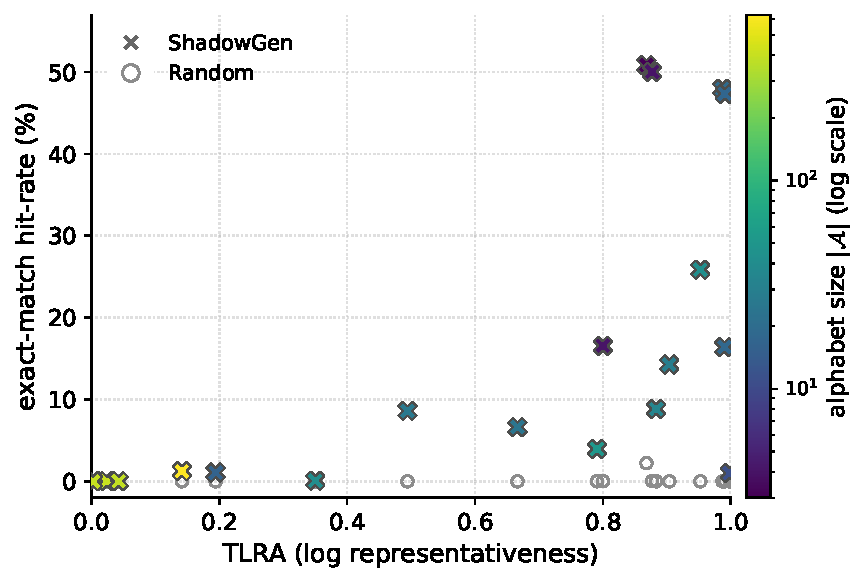
\includegraphics[width=0.62\textwidth]{figures/fig_genval_box.pdf}
\caption{Generator premise across the 21-log catalog: exact-match hit-rate against log representativeness (TLRA), ShadowGen crosses coloured by alphabet size $|\mathcal{A}|$ vs the uniformly random floor (open circles), one point per log. ShadowGen exceeds random on every log (random never above $2.2\%$). Two structural properties shape exact-matchability: hit-rate correlates with representativeness (Pearson $0.66$ with TLRA) and against alphabet size (Pearson $-0.65$ on $\log|\mathcal{A}|$). The floor cluster is the large-alphabet municipality logs ($|\mathcal{A}|$ up to $624$), which are also the least representative, so both properties push them to zero.}
\label{fig:genvalbox}
\end{figure}

\subsubsection{Runtime.}
\label{sec:eval:runtime}
At its default single-draw operating point ($K{=}1$), ShadowGen scores a model in a median of $3$ seconds over all five logs, faster than every published baseline, the next being the trivial PM4Py built-in at $18.6$\,s, which does not track the ground truth. The cost is measured, not projected: timing each cell at both settings puts the $K{=}5$/$K{=}1$ ratio at $5.0\times$, the linear scaling of independent draws. The benchmark reports the $K{=}5$ mean for its error bars (median $14.9$\,s, worst cell $22$ minutes on L4 Inductive-strict); a single draw reproduces it to within Pearson $0.003$ (Sect.~\ref{sec:eval:threats}), so $K$ is a validation knob, not an operating cost. Even at $K{=}5$ ShadowGen is faster than PM4Py, whose worst cell reaches $3.5$ hours. The bootstrap adaptation has the same shape at $2.5\times$ the cost (median $36.9$\,s), and the references are of a different order: R1 reaches a worst cell of $5.7$ hours and leave-one-variant-out $46$ hours. AVATAR exceeds the budget on every log (Sect.~\ref{sec:eval:feasibility}). Figure~\ref{fig:pareto} sets accuracy against time over the whole benchmark. Among methods that agree with the ground truth, ours is the fastest, at $K{=}1$ by roughly sixfold over the next.

\begin{figure}[t]
\centering
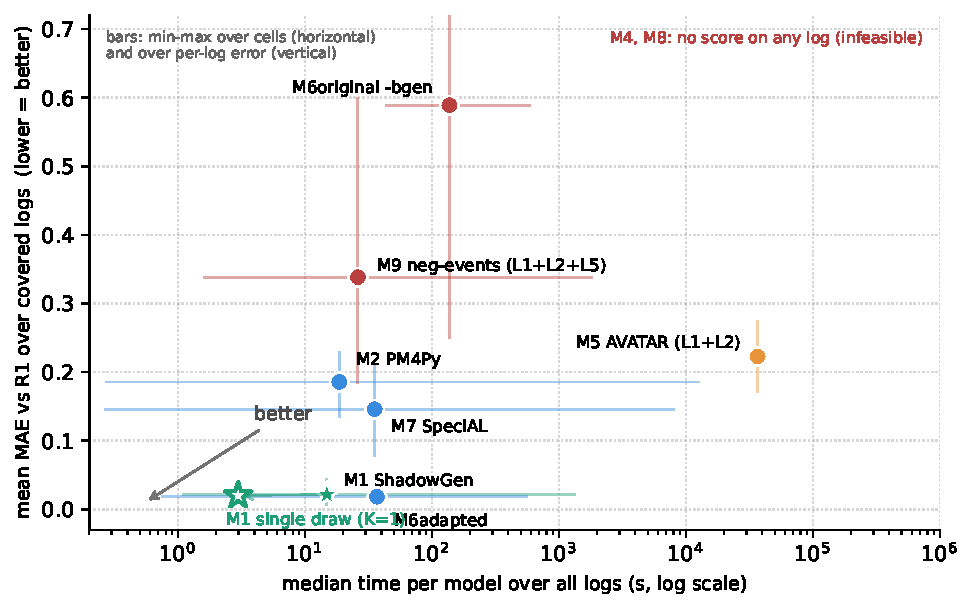
\includegraphics[width=0.85\textwidth]{figures/fig_pareto_scale.pdf}
\caption{Speed against accuracy over all five logs: median time per model (log scale) versus mean of the per-log MAEs to R1; lower-left is better. Whiskers show the spread the aggregates hide: horizontal, min to max cell runtime; vertical, min to max per-log MAE. M1 ShadowGen and M6adapted are alone in the accurate corner; M2 PM4Py is fast but never accurate; M9 negative events is fast but poorly calibrated (plotted on the three logs it covers); the Entropia \texttt{-bgen} F-measure (M6original) is slow and the worst-calibrated method that returns; M5 AVATAR is a budget sentinel on all five logs, plotted at its measured GPU training cost (median ${\sim}10$\,h per log over L1/L2; the CPU projection is $3$--$4$ days; Sect.~\ref{sec:eval:feasibility}) without a time whisker, its accuracy read from the two small logs it scores off-protocol. Partial-coverage points carry their logs in the label. M4 and M8 do not complete a scorable comparison.}
\label{fig:pareto}
\end{figure}

\subsection{Discussion}
\label{sec:eval:discussion}
On five real-life logs spanning $15$ thousand to $2.5$ million events, the methods that confront a model with resampled or synthesized behavior (M1 ShadowGen, M6adapted) agree with the cross-validation ground truth in both rank and absolute value; methods that inspect structure or aggregate diversity (M2 PM4Py, M7 SpeciAL) do not, on any log. This supports the core hypothesis: generalization is a claim about unseen behavior and is best measured by probing models with plausible unseen behavior, not by analysing existing structure. Our metric reaches this agreement at interactive runtime, at $2.5\times$ lower cost than the bootstrap, with interpretable internals (per-context novelty, mutation flags, the openness profile, the acceptance reading) that neural and bootstrap aggregates do not expose. The honest claim is therefore not ``best metric'' but ``matches the strongest baseline's calibration while probing genuinely unseen behavior that resampling cannot reach, and exposing why a model scored as it did, at comparable cost and with no external toolchain.''

\subsection{Threats to validity}
\label{sec:eval:threats}
Seven threats qualify the results; each is stated with what limits it.

\chg{Breadth: the study covers five logs and eight discovery configurations per log, but every correlation is computed over six non-degenerate miners (fewer where flagged), a deliberately small, interpretable sample (an L1 check over eleven configurations gives the same calibration, Sect.~\ref{sec:eval:external}); dataset-specific structure can still favor particular methods, and the AVATAR comparison rests on two off-protocol small-log scorecards, so its verdict is correspondingly limited.}

Shared measurement core: the metric, R1, R3, and M6adapted all score via token replay, so part of their mutual agreement may reflect a shared fitness notion rather than shared generalization semantics. R1's per-fold rediscovery limits but does not eliminate this, and the acceptance reading was validated against a separately computed ground truth (R1-accept). \chg{We also tested the engine directly: recomputing R1 on L1 with cost-zero alignments leaves ShadowGen's ranking unchanged (Spearman $1.0$, Pearson $0.96$ over the five sound nets). Alignment fitness is undefined on unsound nets (the tool refuses Alpha+, which token replay scores), one reason the metric uses token replay.}

Ground truth and representativeness: our validation rests on agreement with variant-based hold-out (R1/R2), the strongest available empirical reference because its test traces are provably valid where a shadow trace is only plausible by construction. Both are computed from the log, so both are only as faithful to the system as the log is representative of it, a responsibility of the data-gathering stage rather than of the metric (Sect.~\ref{sec:related}). \chg{The registered prediction that our calibration error grows as representativeness falls was tested and refuted (Sect.~\ref{sec:eval:scale}); the bound is real, but TLRA alone does not govern it.}

\chg{Generator validity: the premise that the shadow log resembles valid future behavior is tested directly (Sect.~\ref{sec:eval:genval}): up to $25.9\%$ of generated traces are exact held-out real variants, against at most $0.01\%$ for random traces. The residual threat is that exact matching is a lower-bound criterion: on deep-trace logs it cannot certify realism (L4: $0.09\%$), where the premise is supported only indirectly by the graded calibration and by the near-match reading ($2\%$ of L4 traces within three edits of a held-out variant, both floors zero).}

Adapted and incomplete baselines: M6adapted uses token-replay fitness in place of the Entropia precision/recall F-measure\chg{, and its sampler is our reimplementation from the paper, validated on L1} (Sect.~\ref{sec:impl:baselines}); M3 uses a DFG approximation \chg{at scale and a proper reachability SDFA where reachability stays finite ($24$ of $40$ cells across the five logs)} (Sect.~\ref{sec:impl:baselines}); M5 has two of $3$--$5$ planned sampling runs \chg{on its off-protocol L1/L2 scorecards, and its budget sentinels on all five logs are evidence-based (Sect.~\ref{sec:eval:feasibility})}; \chg{M7's L5 cells use a newer package version than L1--L4 (Sect.~\ref{sec:impl:baselines})}; R2 sampled $50$ of $846$ variants on L1\chg{, and the L4 Inductive-strict cell of R2 is sampled at $50$ of $28{,}457$ variants (a full leave-one-variant-out there would need $28{,}457$ rediscoveries)}.

Calibration provenance: $N{=}6$ was originally chosen on one log via a mutation-rate proxy. That criterion is retired: measured directly, the rate rises monotonically with $N$ on every log and offers no maximum (Fig.~\ref{fig:nsweep}). The value survives the direct test, since the five-log sweep re-justifies $N{=}6$ by calibration alone (Sect.~\ref{sec:eval:setup}). The mutated-trace share still varies strongly across logs ($\sim2\%$ of shadow traces on BPI 2017 vs.\ $\sim54\%$ on Sepsis at $N{=}6$), so proposal-distribution effects are dataset-dependent by construction. \chg{Relatedly, the variable-order model's advantage over its 1-gram floor is itself log-dependent: on short, simple logs the 1-gram can match or exceed it (Sect.~\ref{sec:eval:scale}); deep context pays off specifically where decisions depend on it.} \chg{The $\tau$ sensitivity is separately flat: at $N{=}6$, MAE moves by at most $0.007$ across $\tau\in\{2,5,10\}$ (L1 and L3).}

Stochastic stability, measured: the generator's own sampling variance is small and carried in every $\pm$std, so a fixed seed hides no fragility. Across the five independent $1{,}000$-trace draws per cell the score std is at most $0.008$ (median $0.001$), two to three orders of magnitude below the between-model spread it resolves. The metric is in fact single-draw stable: recomputing the four-criteria agreement on each draw separately holds Pearson at or above $0.982$ on every log and reproduces the ranking exactly (draw-to-draw std $\le0.003$ on Pearson, and MAE within $0.007$). This is why the shipped default is a single draw ($K{=}1$): $K{=}5$ is reported for its error bars, not because the result needs averaging.

Replay reproducibility, measured: PM4Py's token replay breaks ties by element iteration order on nets with duplicate labels or silent transitions, and no seed pins it. We measured the drift across independent processes: the trace model moves by up to $0.024$, Alpha+ by up to $0.006$ (on L4), and every other cell reproduces exactly. The four-criteria agreement is essentially unaffected (the worst-case L4 MAE moves from $0.015$ to the tabulated $0.016$), and all discovery-side nondeterminism is pinned (fixed hash seed, models discovered once and cached). The acceptance proxy itself is quantified in Sect.~\ref{sec:eval:accept}.

% =====================================================================
\section{Conclusion}
\label{sec:conclusion}

We presented ShadowGen, a generative N-gram metric for measuring generalization, together with the strict construct definition it implements and a benchmark that validates generalization metrics against variant-based cross-validation under a four-criterion protocol with both construct poles included. The central result: ShadowGen tracks the empirical ground truth on all five real-life logs, reproducing the cross-validation ranking and staying calibrated to it at a median of $3$ seconds per model, faster than every published baseline, while scoring a model artifact in hand, where the cross-validation reference cannot. The benchmark adds findings of independent value: the PM4Py metric is anti-correlated with empirical generalization on four of five logs and fails the flower litmus on all five; two published metrics return on too few models to be scored; AVATAR exceeds the one-hour budget on every log; rank correlation alone is too weak a validation criterion; an independently designed bootstrap generator lands on the same calibration; and the acceptance reading anchors the construct poles while the generator premise is confirmed across the full log catalog.

Open questions remain, and they mark the research opportunities we see. The metric and much of its cross-validation reference share a token-replay core, so part of their agreement reflects a shared conformance notion; an alignment-based acceptance reading would remove the replay proxy and its measured one-sided error, and an alignment-based recomputation of R1 already keeps the ranking (Sect.~\ref{sec:eval:threats}). Per-domain hyperparameter tuning is an open refinement of the fixed-defaults protocol. The strict acceptance reading saturates on deep-trace logs, which invites a graded membership notion for that regime. Several baselines run adapted, degraded, or incomplete; AVATAR has full-configuration GPU runs only on the two smallest logs, and extending them to the large logs would let the second generative paradigm be judged at scale. A proper stochastic-automaton conversion of entropic relevance is not among the open items: we implemented it, and it fails the flower litmus (Sect.~\ref{sec:eval:feasibility}). The metric itself is feature-frozen; the name ShadowGen reflects its purely generative design.

% =====================================================================
% DECLARATION ON THE USE OF AI-BASED TOOLS
% No Informatics-specific template found; using a one-line declaration.
% Revisit if the chair requires a specific format or a per-author tool list.
% =====================================================================
\section*{Declaration on the Use of AI-Based Tools}
In preparing this work, we used AI-based assistants (large-language-model and coding
tools) for source-code drafting, figure generation, and language editing; all content
was reviewed and verified by the authors, who take full responsibility for it.

% =====================================================================
\appendix
\section{Acceptance-reading agreement}
\label{sec:appendix:accept}
Table~\ref{tab:accept} gives the per-miner acceptance detail on L1 (\genaccept{} vs the acceptance ground truth R1-accept); Table~\ref{tab:accept-scale} reports the per-log agreement, the acceptance companion to the graded-fitness scale table (Table~\ref{tab:scale}). Both back Sect.~\ref{sec:eval:accept}.

\begin{table}[h]
\centering
\caption{Acceptance reading on L1 (\genaccept) vs the acceptance ground truth (R1-accept), per miner.}
\label{tab:accept}
\setlength{\tabcolsep}{3.5pt}
\footnotesize
\begin{tabular}{@{}lcccccccc@{}}
\toprule
 & Trace & Alpha & Alpha$+$ & Heur. & Heur.S & Ind.Inf & Ind.S & Flower \\
\midrule
\genaccept{} & .000 & .000 & .000 & .001 & .008 & .644 & .744 & 1.00 \\
R1-accept & .000 & .000 & .000 & .028 & .043 & .783 & .996 & 1.00 \\
\bottomrule
\end{tabular}
\end{table}

\begin{table}[h]
\centering
\caption{Acceptance reading (\genaccept) vs the acceptance ground truth (R1-accept): agreement over the six non-degenerate miners per log, plus the two construct poles. Both anchor the trace and flower poles at $0$ and $1$ on every log (largest deviation $0.003$, the L5 trace model; Sect.~\ref{sec:eval:accept}). $^{*}$Pearson is uninformative on L4: strict acceptance saturates at trace depth (mean $57$ events), leaving only two mid-range cells with signal (Sect.~\ref{sec:eval:accept}).}
\label{tab:accept-scale}
\setlength{\tabcolsep}{6pt}
\footnotesize
\begin{tabular}{@{}lrrc@{}}
\toprule
Log & Pearson & MAE & Poles (Trace\,/\,Flower) \\
\midrule
L1 Sepsis   & 0.998 & 0.076 & 0.00\,/\,1.00 \\
L2 BPI 2013 & 0.997 & 0.021 & 0.00\,/\,1.00 \\
L3 BPI 2017 & 0.992 & 0.039 & 0.00\,/\,1.00 \\
L4 BPI 2018 & \emph{n/a}$^{*}$ & 0.057 & 0.00\,/\,1.00 \\
L5 BPI 2019 & 0.999 & 0.075 & 0.00\,/\,1.00 \\
\bottomrule
\end{tabular}
\end{table}

\section{Raw cross-paradigm scores on L1}
\label{sec:appendix:external}
\chg{Table~\ref{tab:external} gives the full per-cell scores behind the L1 calibration (Sect.~\ref{sec:eval:external}): the metrics of the L1 comparison and the cross-validation references on each of the seven miners. It is the numeric backing for Figure~\ref{fig:calibration} and Table~\ref{tab:corr}; the R3-Random row is the construct floor made concrete, collapsing in the mid-permissiveness cells ($.502$, $.621$) where the real ground truth ($.902$, $.933$) does not.}

\begin{table}[h]
\centering
\caption{L1 Sepsis: scores per miner, mean $\pm$ std where applicable (seven miners of the external comparison). $^{\ddagger}$model fitness $<0.5$ on the log. $^{\dagger}$returns too few comparable cells (Sect.~\ref{sec:eval:feasibility}). \chg{\textsuperscript{\S}off-protocol budget sentinel (Sect.~\ref{sec:eval:feasibility}): shown for the litmus and Fig.~\ref{fig:calibration}, excluded from the agreement statistics.}}
\label{tab:external}
\setlength{\tabcolsep}{1.6pt}
\scriptsize
\begin{tabular}{@{}lccccccc@{}}
\toprule
Method & Alpha$^{\ddagger}$ & Alpha$+$ & Heur. & Heur.S & Ind.Inf & Ind.S & Flower \\
\midrule
\chg{ShadowGen (ours)} & .272$\pm$.004 & .759$\pm$.005 & .879$\pm$.002 & .917$\pm$.002 & .972$\pm$.002 & .984$\pm$.002 & 1.00 \\
M2 PM4Py & .913 & .919 & .830 & .900 & .880 & .902 & .913 \\
M5 AVATAR\chg{\textsuperscript{\S}} & .329$\pm$.057 & .312$\pm$.002 & .746$\pm$.063 & .734$\pm$.110 & .697$\pm$.021 & .571$\pm$.023 & .330$\pm$.007 \\
M6adapted$^{*}$ & .250$\pm$.010 & .775$\pm$.018 & .891$\pm$.003 & .930$\pm$.003 & .976$\pm$.003 & .994$\pm$.001 & 1.00 \\
M7 SpeciAL & .799 & .750 & 1.00 & .998 & .750 & .744 & .803 \\
M4 Anti-align.$^{\dagger}$ & \multicolumn{7}{c}{\emph{two of seven L1 cells, anti-alignment scale, not comparable}} \\
M8 Pattern$^{\dagger}$ & \multicolumn{7}{c}{\emph{no L1 cell within the hour}} \\
\midrule
R1 5-fold CV & .275$\pm$.001 & .829$\pm$.002 & .902$\pm$.005 & .933$\pm$.001 & .985$\pm$.002 & 1.00 & 1.00 \\
R2 LOVO & .306$\pm$.075 & .775$\pm$.177 & .870$\pm$.051 & .917$\pm$.044 & .981$\pm$.053 & 1.00 & 1.00 \\
R3 Random & .278$\pm$.004 & .382$\pm$.004 & .502$\pm$.005 & .621$\pm$.003 & .693$\pm$.001 & .767$\pm$.002 & 1.00 \\
\bottomrule
\end{tabular}\\[2pt]
{\scriptsize $^{*}$M6adapted scores the genuine \texttt{bsgen} bootstrap sample by token-replay fitness (a graded model--system recall, the construct the bootstrap paper defines~\cite{polyvyanyy2022bootstrap}), not the Entropia \texttt{-bgen} precision/recall F-measure (Sect.~\ref{sec:impl:baselines}). $^{\dagger}$M4 returns two L1 cells (Alpha, Heuristics-strict) as anti-alignment scores, not on this table's fitness scale, and exceeds the hour or aborts on the rest; M8 returns no L1 cell within the hour.}
\end{table}

\section{The bootstrap contamination reading}
\label{sec:appendix:m6}
Table~\ref{tab:m6} is the numeric backing for the controlled bootstrap study of Sect.~\ref{sec:eval:m6}: one bred \texttt{bsgen} sample on L1, scored four ways against R1. Only the readings free of precision pass the flower litmus.

\begin{table}[h]
\centering
\caption{The same \texttt{bsgen} bootstrap sample on L1, scored four ways, vs R1 (six non-degenerate miners). Only the readings free of precision pass the flower litmus.}
\label{tab:m6}
\setlength{\tabcolsep}{5pt}
\footnotesize
\begin{tabular}{@{}lrrrrl@{}}
\toprule
Reading of the bootstrap sample & Pearson & $\tau_b$ & MAE & Flower & litmus \\
\midrule
M6original \texttt{-bgen} F1(prec, rec) & 0.87 & 0.20 & 0.59 & 0.18 & fail \\
\quad its precision component & 0.82 & 0.20 & 0.68 & 0.10 & fail \\
\quad its \textbf{recall} component & 0.98 & 0.73 & 0.11 & 1.00 & pass \\
\textbf{M6adapted} (token-replay) & 1.00 & 1.00 & 0.018 & 1.00 & pass \\
\bottomrule
\end{tabular}
\end{table}

\section{Feasibility forensics}
\label{sec:appendix:feasibility}
This section records the full per-method evidence behind the feasibility verdicts of Sect.~\ref{sec:eval:feasibility} (Table~\ref{tab:feasibility}).

\emph{M4 and M8.} Anti-alignments (M4) run the published implementation~\cite{vandongen2016anti} under the same budget. It scores three of the eight L1 models and three of the eight L2 models, never more than two of the six non-degenerate miners, nothing on L3 or L4, and only the trace pole on L5; on L4 the $2.5$ million event log does not finish even the alignment step within the hour. On L1 Inductive-infrequent aborts inside the solver on an internal index overflow, Alpha+ reaches $1\%$ of its traces within the hour, Heuristics reaches $87\%$ at the kill (the one near-miss) and Inductive-strict $0.1\%$, and the flower model never returns. Where M4 does score, the trace model reads $0.0$, the correct pole. Pattern-based generalization (M8)~\cite{reissner2022pattern} fails similarly: it scores three of the eight L2 models in seconds (Heuristics $0.99$, Heuristics-strict $0.999$, and the trace model), crashes with a null alignment on the other five, and returns nothing on L1, L3, L4, or L5. Unlike M4, it exposes no progress counter, so its non-returns are wall-clock kills without a measured progress percentage. Its $0.90$ on the trace model is the wrong pole, a memorizing model read as general. Neither returns all six non-degenerate miners on any log, so neither can be placed on the four-criteria agreement.

\emph{M3.} Entropic relevance is feasible on all five logs as a directly-follows approximation (Sect.~\ref{sec:impl:baselines}), but its agreement with the ground truth is unstable (per-log Pearson against R1 from $-0.80$ to $+0.95$), so we do not read it as tracking held-out fitness. Computed properly, from a stochastic automaton built from each net's reachability graph, it confirms the problem directly: on L1 two of the six non-degenerate miners (Alpha, Heuristics) have no finite automaton, and on the four that convert it places the flower model mid-field ($52$ bits against $22$ to $62$ for the real models), failing the flower litmus. Extended to all five logs, the proper conversion builds on $24$ of $40$ cells (all $8$ on the $4$-activity L2, $3$ of $8$ on L5, at a $150$k-marking cap); the deeper the concurrency, the fewer nets convert. Entropic relevance scores a fitness and precision blend, not generalization, so we keep it out of the agreement tables.

\emph{M9.} Negative-event generalization~\cite{vandenbroucke2014negative}, run through the CoBeFra implementation in its shipped configuration (weighted artificial negatives with token replay), does not track held-out generalization on any log. On L1 it is anti-correlated with the ground truth over the six non-degenerate miners (Pearson $-0.55$, more negative than PM4Py), rating the well-generalizing Heuristics models near zero; on the four-activity L2 and the short-trace L5 it collapses, scoring every model $1.0$ including the memorizing trace pole, so it discriminates nothing (MAE $0.18$ and $0.23$). It passes the flower litmus on the small logs ($1.0$) but mis-anchors the trace pole ($0.48$ on L1, $1.0$ on L2 and L5), and it does not scale: on L3 only two of the six non-degenerate miners return within the hour and on L4 (mean trace length $57$) none do. Its scores are also non-deterministic on nets with silent transitions (L1 Inductive-infrequent, std $0.07$ across runs), the same token-replay tie-breaking that affects the acceptance proxy (Sect.~\ref{sec:eval:accept}). Because it is degenerate on L2 and L5 and infeasible at scale on L3 and L4, no scorable four-criteria result exists. The run and driver are in \texttt{benchmark/m9/}.

\emph{M5.} AVATAR's two small-log scorecards are obtained off-protocol (two of the $3$--$5$ published runs). The cost evidence is measured on both hardware classes. On GPU, the full published configuration ($100$ pre-epochs, $5{,}000$ adversarial steps) needs $11.8$ hours of training on L1 and $8.6$ on L2, an order of magnitude past the budget on the two smallest logs, consistent with the authors' reported training times~\cite{theis2020avatar}. On benchmark-class CPU, a reduced L1 anchor ($3$ of $100$ pre-epochs, $100$ of $5{,}000$ adversarial steps) already needs $88$ minutes, and its per-step rate ($45$\,s) projects the full configuration to ${\sim}3$--$4$ days per log (over $400$ CPU-hours); L3 spent its full CPU hour without leaving GAN pretraining, and L4 was killed at both a $16$ and a $24$\,GB memory cap. Its published configuration also caps sequences at $20$ events, below the mean trace length of L3 ($38.2$) and L4 ($57.4$), so its scores there would truncate the behavior generalization asks about; raising the cap is a configuration change that only adds to the already prohibitive cost.

\section{Per-method calibration across the five logs}
\label{sec:appendix:calibration}
Figure~\ref{fig:calibration} is the visual companion to Table~\ref{tab:scale}: every metric against the ground truth, all five logs in one panel per method.

\begin{figure}[h]
\centering
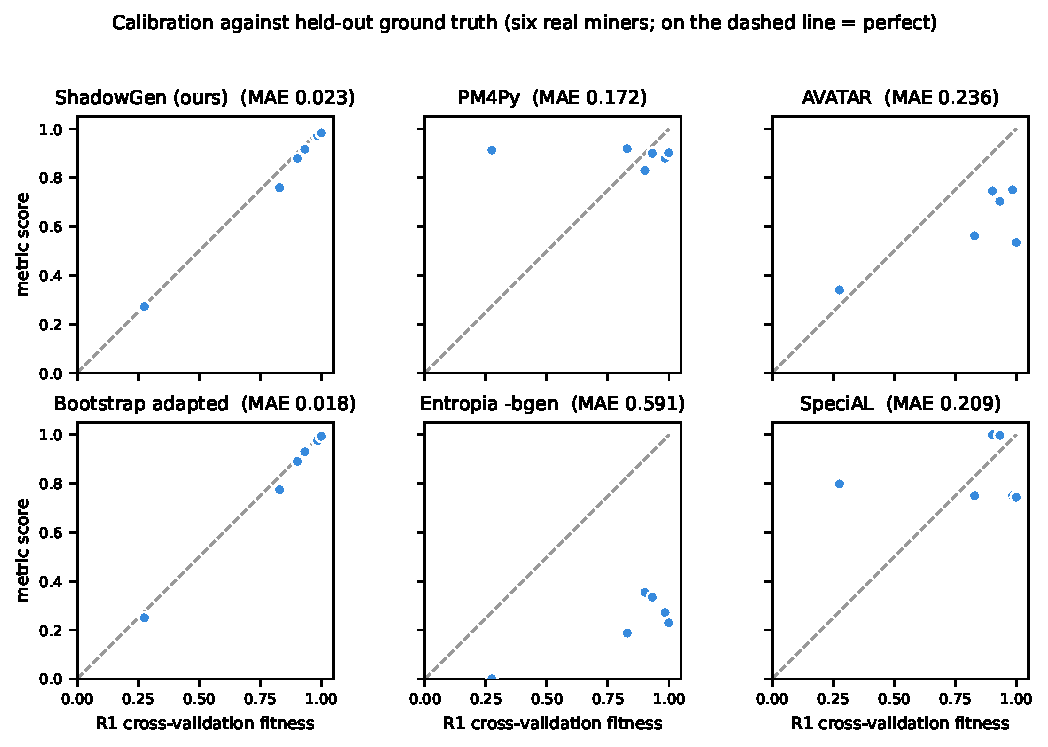
\includegraphics[width=0.86\textwidth]{figures/fig_calibration_d1v2.pdf}
\caption{Per-method calibration against the cross-validation ground truth R1 across all five logs (six non-degenerate miners per log, up to 30 points, one marker per log; dashed line $y{=}x$). The generative and resampling metrics (M1 ShadowGen, M6adapted) sit on the line on every log; the published Entropia \texttt{-bgen} F-measure of the same bootstrap sample (M6original) sits far below it (its F1 folds precision in, Sect.~\ref{sec:eval:m6}); M2 PM4Py forms a flat band that ignores the ground-truth gradient; M5 AVATAR (shown off-protocol on L1/L2 only, Sect.~\ref{sec:eval:feasibility}) and M7 SpeciAL scatter off the line. Metrics that could not run on every log appear with fewer points: AVATAR's sparse panel is itself the feasibility verdict.}
\label{fig:calibration}
\end{figure}

\begin{figure}[h]
\centering
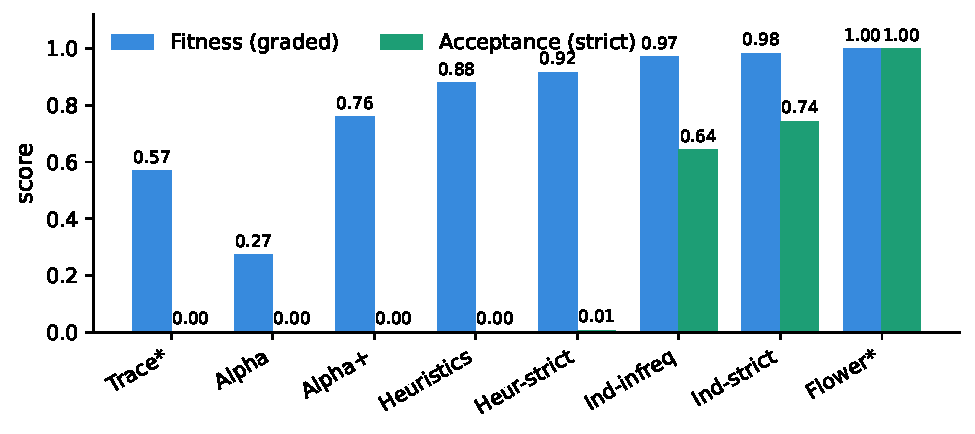
\includegraphics[width=0.72\textwidth]{figures/fig_accept_d1.pdf}
\caption{Two readings of the shadow log on L1 Sepsis: graded fitness (partial credit) vs.\ strict acceptance (perfect-replay fraction). Acceptance gives the construct's clean poles (Trace $0.00$, Flower $1.00$), and the gap between the bars exposes partial-credit inflation: e.g.\ Alpha+ scores $0.76$ fitness but $0.00$ acceptance, and the trace model $0.57$ fitness but $0.00$ acceptance (Sect.~\ref{sec:eval:accept}).}
\label{fig:accept}
\end{figure}

\section{Generator premise per log}
\label{sec:appendix:genval}
Table~\ref{tab:genval} gives the per-log exact-match rates behind Sect.~\ref{sec:eval:genval}.

\begin{table}[h]
\centering
\caption{Generator premise: share of generated traces that exactly match held-out real variants (mean over $15$ folds, in \%), and the share of the held-out variant set reached (coverage, in \%). TLRA (trace-based log representativeness, Table~\ref{tab:datasets}) is repeated here: the hit-rate tracks it at Pearson $0.97$.}
\label{tab:genval}
\setlength{\tabcolsep}{5pt}
\footnotesize
\begin{tabular}{@{}lrrrrr@{}}
\toprule
Log & TLRA & ShadowGen & 1-gram & Random & Coverage \\
\midrule
L1 & 0.19 & 1.1 & 0.4 & 0.0 & 4.8 \\
L2 & 0.80 & 16.6 & 10.9 & 0.01 & 10.6 \\
L3 & 0.49 & 8.6 & 0.0 & 0.0 & 1.4 \\
L4 & 0.35 & 0.09 & 0.0 & 0.0 & 0.01 \\
L5 & 0.95 & 25.9 & 5.5 & 0.0 & 1.7 \\
\bottomrule
\end{tabular}
\end{table}

\section{Baseline integration details}
\label{sec:appendix:baselines}
The engineering record behind Sect.~\ref{sec:impl:baselines}. SpeciAL (M7) is a Python package used directly; on L5 we use the released PyPI package (\texttt{special4pm} 0.1.3), on L1--L4 the source copy provided by the authors' repository, a version skew we disclose (Sect.~\ref{sec:eval:threats}). Entropic relevance (M3) needs a Petri-net-to-stochastic-automaton conversion, reported two ways. At scale we approximate it with a per-miner DFG simulation (PM4Py \texttt{play\_out}, 5\,000 traces) converted to a probability automaton via the open-source \texttt{relevance.jar} from the Entropia toolset~\cite{polyvyanyy2020entropia} (JDFG2Aut + Relevance); this runs on all five datasets but takes its transition probabilities from the simulated DFG frequencies, not from the net. For the construct test we build the automaton properly, from each net's reachability graph with silent transitions collapsed and the result determinized over visible labels, probabilities from log replay, scored with Entropia's entropic relevance directly. The proper conversion is exact but bounded (Appendix~\ref{sec:appendix:feasibility}). Both are additionally reimplemented in plain Python and validated against the Entropia tool ($3$-decimal agreement on every L1 automaton). For M6, our bridge runs the genuine \texttt{bsgen} bootstrap-with-breeding sampler and scores the bred traces by PM4Py token-replay fitness, a graded model--system recall, the way \genshadow{} grades the shadow log; the sampler is our reimplementation of the paper's published algorithms (the original source is not public) and reproduces the published L1 values within $0.008$ on every cell.

\section{Choosing the context bound}
\label{sec:appendix:nsweep}
Figure~\ref{fig:nsweep} is the five-log sweep behind the $N{=}6$ default (Sect.~\ref{sec:eval:setup}).

\begin{figure}[h]
\centering
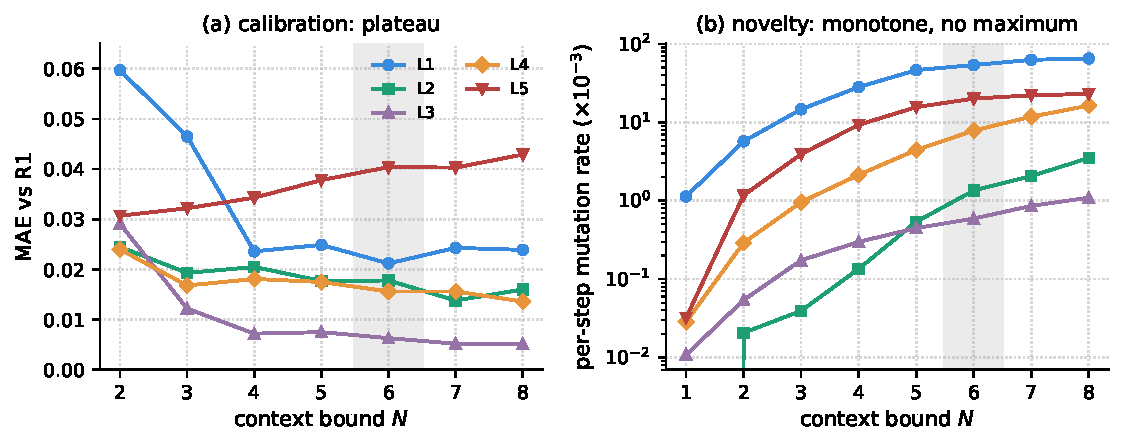
\includegraphics[width=0.95\textwidth]{figures/fig_nsweep.pdf}
\caption{Choosing the context bound $N$, swept on all five logs ($\tau{=}5$, $K{=}1$). (a) MAE to R1 plateaus from $N{\approx}4$ on every log; $N{=}6$ is optimal on L1 and within $0.004$ on L2--L4. (b) The realized per-step mutation rate rises monotonically with $N$ on every log (log scale) and offers no maximum, so calibration, not novelty, fixes $N$. The band marks the chosen $N{=}6$.}
\label{fig:nsweep}
\end{figure}

\section{Complexity derivation}
\label{sec:appendix:complexity}
Let $|V(L)|$ be the number of variants, $E_V=\sum_{v\in V(L)}|v|$ the summed length of the variants, $A=|\mathcal{A}|$ the alphabet size, $N$ the context bound, $\theta$ the shadow-log size, and $K$ the iteration count. Let $\ell_{\max}=\max_{v\in V(L)}|v|$ be the length of the longest variant; the walk cap is set data-driven to $\lambda\approx2\ell_{\max}$. Let $|M_P|$ be the size of the Petri net under evaluation, measured as its number of places, transitions, and arcs. Building the N-gram statistics is $O(N\,E_V)$ in time and $O(N\,G)$ in space for the $G$ stored distinct $n$-grams. Generation is $O(\theta\,\lambda\,\bar b)$ with mean branching factor $\bar b\le A$, since context resolution and termination are memoized on the last $N$ activities, so each distinct context is resolved once. Token replay is roughly linear in trace length and net size~\cite{rozinat2008conformance}, $O(\theta\,\lambda\,|M_P|)$. Per evaluated model the total is $O\!\big(K\,(N\,E_V + \theta\,\lambda\,\bar b + \theta\,\lambda\,|M_P|)\big)$. The leave-one-variant-out ground truth performs $|V(L)|$ full discoveries, $O(|V(L)|\cdot\mathrm{discover})$.

\section{Katz mutation at realistic counts}
\label{sec:appendix:mutation}
Figure~\ref{fig:mutation} illustrates the two-job split of backoff (Sect.~\ref{sec:method:gen}) at realistic successor counts.

\begin{figure}[h]
\centering
\scalebox{0.82}{%
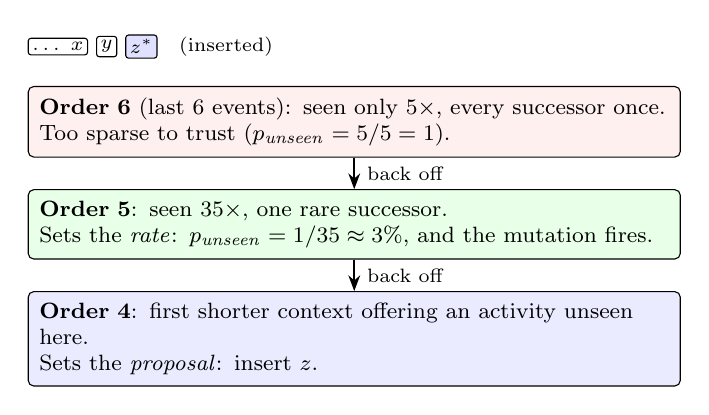
\begin{tikzpicture}[
  font=\footnotesize, node distance=4mm,
  lvl/.style={draw, rounded corners=2pt, align=left, inner sep=4pt, text width=80mm},
  ev/.style={draw, rounded corners=1pt, font=\scriptsize, inner sep=1.5pt},
  arr/.style={-{Stealth[length=2mm]}, semithick}
]
\node[ev] (a) {$\dots\ x$};
\node[ev, right=1mm of a] (b) {$y$};
\node[ev, right=1mm of b, fill=blue!12] (c) {$z^{*}$};
\node[right=1.5mm of c, font=\scriptsize] {(inserted)};
\node[lvl, fill=red!6, below=5mm of a.west, anchor=north west] (n6)
  {\textbf{Order 6} (last 6 events): seen only $5\times$, every successor once.\\
   Too sparse to trust ($\punseen=5/5=1$).};
\node[lvl, fill=green!9, below=of n6] (n5)
  {\textbf{Order 5}: seen $35\times$, one rare successor.\\
   Sets the \emph{rate}: $\punseen=1/35\approx3\%$, and the mutation fires.};
\node[lvl, fill=blue!8, below=of n5] (n4)
  {\textbf{Order 4}: first shorter context offering an activity unseen here.\\
   Sets the \emph{proposal}: insert $z$.};
\draw[arr] (n6) -- node[right=1pt,font=\scriptsize]{back off} (n5);
\draw[arr] (n5) -- node[right=1pt,font=\scriptsize]{back off} (n4);
\end{tikzpicture}}
\caption{Katz-consistent mutation at realistic counts (illustrative; activities abstracted to $x,y,z$). Backoff sets both \emph{how often} to invent an event (the rate, resolved at order~5) and \emph{what} to invent (the proposal, found at order~4): novel in the exact context, yet attested in a related shorter one.}
\label{fig:mutation}
\end{figure}

\bibliographystyle{splncs04}
\bibliography{references}

\end{document}
